%% $Id:  $
%% $HeadURL:  $
\documentclass{llncs}

\usepackage[T1]{fontenc}
\usepackage{microtype}
\usepackage[utf8]{inputenc}
\usepackage{amsmath,amssymb}
\usepackage[lighttt]{lmodern}
\usepackage{helvet,times,courier}
\usepackage{xcolor}
\usepackage{graphicx}
\usepackage{listings}
\AtBeginDocument{\DeclareCaptionSubType{lstlisting}}
\usepackage{caption,subcaption}
\usepackage{hyperref}
\usepackage{tikz}
\lstset{xleftmargin=2\parindent,aboveskip=\smallskipamount,belowskip=\smallskipamount,captionpos=b}
\lstset{numbers=left,numberblanklines=false,basicstyle=\ttfamily}

\lstdefinelanguage{clingo}{
  keywordstyle=[1]\usefont{OT1}{cmtt}{m}{n},%
  keywordstyle=[2]\textbf,%
  keywordstyle=[3]\usefont{OT1}{cmtt}{m}{n},%\textit
  alsoletter={\#,\&},%
  keywords=[1]{not,from,import,def,if,else,elif,return,while,break,and,or,for,in,del,and,class,with,print,as,is},%
  keywords=[2]{\#const,\#show,\#minimize,\#base,\#theory,\#count,\#external,\#program,\#script,\#end,\#heuristic,\#edge,\#project,\#show,\#sum},%
  keywords=[3]{&,&dom,&sum,&diff,&show},%
  morecomment=[l]{\#\ },%
  morecomment=[l]{\%\ },%
  morestring=[b]",%
  stringstyle={\textit},%
  commentstyle={\color{darkgray}}%
}

\newcommand{\gringo}{\textit{gringo}}
\newcommand{\clasp}{\textit{clasp}}
\newcommand{\clingo}{\textit{clingo}}
\newcommand{\asprin}{\textit{asprin}}
\newcommand{\asap}{\textit{teaspoon}}
\newcommand{\piclasp}{\textit{piclasp}}

\newcommand{\code}[1]{\lstinline[basicstyle=\ttfamily]{#1}}

\newcommand{\lw}[1]{\smash{\lower1.ex\hbox{#1}}}
\newcommand{\llw}[1]{\smash{\lower3.ex\hbox{#1}}}

%\newcommand{\dataCL}[5]{%
%  \code{#1} & #3 & #5 & #4
%}
%\newcommand{\dataCS}[5]{%
%  #3 & #5 & #4
%}

\newenvironment{tableC}{%
  \scriptsize
  \tabcolsep = 0.6mm
  \begin{tabular}[t]{l|rlr|rlr|rlr|rlr|rlr}\hline
    \multicolumn{1}{l|}{\llw{Instance}} &
    \multicolumn{3}{c|}{UD1} &
    \multicolumn{3}{c|}{UD2} &
    \multicolumn{3}{c|}{UD3} &
    \multicolumn{3}{c|}{UD4} &
    \multicolumn{3}{c}{UD5} \\
    & 
    \multicolumn{1}{c}{Best} & & \multicolumn{1}{c|}{\emph{tea-}} & 
    \multicolumn{1}{c}{Best} & & \multicolumn{1}{c|}{\emph{tea-}} & 
    \multicolumn{1}{c}{Best} & & \multicolumn{1}{c|}{\emph{tea-}} & 
    \multicolumn{1}{c}{Best} & & \multicolumn{1}{c|}{\emph{tea-}} & 
    \multicolumn{1}{c}{Best} & & \multicolumn{1}{c}{\emph{tea-}} \\
    & 
    known & & \emph{spoon} & 
    known & & \emph{spoon} & 
    known & & \emph{spoon} & 
    known & & \emph{spoon} & 
    known & & \emph{spoon} \\
    \hline
  }{%
    \hline
  \end{tabular}
}

\newenvironment{tableB}{%
  \scriptsize
  \tabcolsep = 0.7mm
%  \begin{tabular}[t]{|l|c|r|l|l|l|}\hline
  \begin{tabular}[t]{lcrlll}\hline
    Instance &
    Formulation &
    Time (sec.)\\
    \hline
  }{%
    \hline
  \end{tabular}
}
\newenvironment{tableL}{%
  \scriptsize
  \tabcolsep = 0.7mm
  \begin{tabular}[t]{l|rrrrrrrr|r}\hline
    \lw{Instance} &
    \lw{Time (sec.)} &
    \multicolumn{6}{c}{The best utility vector} &
    The sum of  &
    The best of basic\\
    &
    &
    $(S_1,$ & $S_4,$ & $S_2,$ & $S_7,$ & $S_6,$ & $S_3)$ &
    utility vector &
    and optimized \\
    \hline
  }{%
    \hline
  \end{tabular}
}

%%% Local Variables:
%%% mode: latex
%%% TeX-master: "paper"
%%% End:
 

\title{A Tutorial on Hybrid Answer Set Solving with \clingo}

\author{%
  Roland Kaminski\inst{1}
  \and
  Torsten Schaub\inst{1,2}\thanks{Affiliated with the
                              School of Computing Science at
                              Simon Fraser University,
                              Burnaby, Canada,
                              and the
                              Institute for Integrated and Intelligent Systems
                              at
                              Griffith University,
                              Brisbane, Australia.}
  \and                            
  Philipp Wanko\inst{1}
  }

\institute{University of Potsdam, Germany \and Inria, Bretagne Atlantique, Rennes}

\begin{document}

\maketitle

%\begin{abstract}
%	The design space for highly complex system level specifications of embedded systems is enormous as tasks may be mapped to different resources and messages may be routed over several links of the hardware platform. 
%	Furthermore, highly constrained requirements lead to many infeasible solutions that have to be sorted out. \emph{\ac{ASP}} in combination with variant background theories (\emph{\ac{ASPmT}}) has been shown to cope with such requirements very efficiently. However, especially in system level design, a fast \emph{\ac{DSE}} including optimization is crucial in order to steer the development towards optimal design points. In this paper, we therefore propose to couple the highly efficient constraint solving capabilities of \ac{ASP} with a \ac{DSE} including \emph{multi-objective optimization} in an additional background theory. Utilizing the possibility to work on \emph{partial assignments}, \ac{ASPmT} is able to prune entire infeasible and dominated regions from the search space early in the decision process. In the experimental section, we present and compare variant approaches and domain specific heuristics.
%\end{abstract}

\begin{abstract}
	An efficient \emph{\ac{DSE}} is imperative for the design of modern, highly complex embedded systems in order to steer the development towards optimal design points. The early evaluation of design decisions at system-level abstraction layer helps to find promising regions for subsequent development steps in lower abstraction levels by diminishing the complexity of the search problem. In recent works, symbolic techniques, especially \ac{ASPmT}, have been shown to find feasible solutions of highly complex system-level synthesis problems with non-linear constraints very efficiently. In this paper, we present a novel approach to a holistic system-level \ac{DSE} based on \ac{ASPmT}. To this end, we include additional background theories that concurrently guarantee compliance with hard constraints and perform the simultaneous optimization of several design objectives. %First experimental results show the applicability of our approach. %for large optimization of up to 170 tasks mapped to 3-dimensional hardware platforms. Furthermore, it outperforms current multi-objective optimization strategies of \ac{ASP} with respect to both diversity and convergence of found solutions.   %We present and investigate several strategies that show the applicability of our approach even for large problem instances. 
	We implement and compare our approach with a state-of-the-art preference handling framework for \ac{ASP}. Experimental results indicate that our proposed method produces better solutions with respect to both diversity and convergence to the true Pareto front.
\end{abstract}

\section{Introduction}
\label{sec:introduction}
%In order to cope with the ever-increasing complexity of embedded systems, system level description are utilized to diminish the complexity of finding potentially good solutions which can then be used as initial starting points for further optimization in lower abstraction levels. On system level, applications are composed of granular tasks that exchange information over communication messages and form dependency relations between each other. The hardware architecture contains heterogeneous processing elements (e.g.~CPU, DSP, GPU) as well as a communication infrastructure like routers and links. Yet, the design space for such system level specifications of embedded systems is still enormous as tasks may be mapped to different computational resources and messages may be routed over several links of the communication infrastructure.\par 
%Furthermore, various hard constraints like maximum latency and energy consumption of the resulting systems have to be considered. That is, only a subset of all possible decisions leads to valid system implementations that conform to previously defined constraints which makes it even hard\footnote{In fact, the mapping problem is known to be $\mathcal{NP}$-hard \cite{Blickle1998}.} to find \emph{one} feasible solution. However, by encoding the problem symbolically (cf.~\cite{Haubelt2003}) and due to the technological advances in \ac{SAT}, various constraint solvers can be utilized to cope with the complexity. Especially, \emph{\acf{ASP}} has been shown to deal with such stringently constrained design problems very efficiently (e.g.~\cite{Andres2013}). Opposed to other symbolic techniques like \ac{SAT}, reachability can be expressed naturally in \ac{ASP} which fastens the routing sub-problem.\par 
%%\ac{ASP} stems from the area of knowledge representation and reasoning and is based on the \emph{stable model semantics}. 
%Finding one feasible solution is however often insufficient. Depending on the decisions that have been made, the qualitative properties (e.g.~latency, energy consumption, area requirements) of the resulting system implementation may vary considerably from solution to solution. Thus, a \acf{DSE} is imperative to find solutions with optimal properties. Usually, the objectives (i.e.~optimizing the individual properties) of \acp{MOOP} are conflicting with each other and no single optimal solution but a set of \emph{Pareto optimal} solutions exists. A Pareto optimal solution is characterized by the property that it is not dominated by (i.e.~not worse in all objectives than) any other solution. \par%That is, all Pareto optimal solutions are mutually non-dominated.\par 
%Commonly, meta-heuristics like \acp{MOEA} are utilized to solve \acp{MOOP}. They are based on natural processes and work on sets of solutions (populations) concurrently. Each solution is evaluated by a fitness function with respect to the objectives and the best solutions are combined to create novel solutions for subsequent generations. As the initial population is created by a randomized process, finding feasible solutions becomes a problem for stringently constraint environments. Moreover, because the search is generally not executed systematically but based on combining previously found solutions, \acp{MOEA} tend to run into saturation and stop finding novel solutions after an arbitrary number of iterations.\par
%In the paper at hand, we therefore propose an approach that utilizes an exact symbolic encoding for both the constraint solving and the design space exploration. Based on \ac{ASP}, we tightly integrate background theory solvers, known as \ac{ASPmT}, that handle (non-)linear objectives as well as Pareto filtering of found solutions. Furthermore, they are able to work on partial solutions to prune the search space from infeasible and dominated regions of design points early in the decision process. 
%The contribution of this paper is threefold:
%\begin{enumerate}
%	\item We present a universal framework for preference handling that is capable of both linear and non-linear objectives based on \ac{ASPmT}.
%	\item In order to combine various background theories for multi-objective optimization and constraint solving concurrently, we present various approaches.
%	\item Extensive experimental test instances show the advantages and disadvantages of the different approaches. 
%\end{enumerate}\par
%\textbf{Paper organization:} Related work will be covered in Sec.~\ref{sec:relatedwork}. Afterwards, the execution model that will be used throughout the paper is briefly described in Sec.~\ref{sec:model}. Section \ref{sec:framework} contains detailed information about our proposed preference handling framework. Experimental results are given in Sec.~\ref{sec:experiments} before Sec.~\ref{sec:conclusion} concludes the paper.

%Essentially, there are three approaches to explore the design space \cite{Pimentel2017}: First, meta-heuristics like evolutionary algorithms have been studied thoroughly in the past (e.g.~\cite{1,2,3,4,5}). Those techniques are inspired by the natural selection process and work on whole sets of solutions (populations) concurrently. Each solution is evaluated and the best are combined to create new solutions for the following generations. One major problem arises if, due to various hard constraints, only a small subset of design points is feasible. Because of their random nature, pure meta-heuristics tend to fail in finding feasible regions of the design space. \par 
%Therefore, the second approach type combines meta-heuristics with exact methods (e.g.~\cite{Neubauer2016,Haubelt2003,Lukasiewycz2012a}). That is, not the decision variables themselves but the heuristics that are used by the constraint solver are subject to the randomized exploration process. Every found design point is thereby guaranteed to be feasible.\par 
%Finally, exact methods have been developed to explore the design space systematically. While meta-heuristics normally only cover a limited portion of the design space, exact methods (e.g.~\cite{6,7,8,9}) such as \ac{ILP} and branch-and-bound algorithms are guaranteed to find the optimal solutions. \par
%However, the latter are often infeasible for real-world problems as the design space is simply too vast to evaluate every design point.
%However, finding even \emph{one} feasible solution that conforms to all constraints is an $\mathcal{NP}$-hard problem (cf.~\cite{Blickle1998}).
%One way to cope with such complexities is to represent such problems symbolically and utilize specialized solvers like \ac{SAT} (e.g.~\cite{Neubauer2016}), \ac{ILP} (e.g.~\cite{Lukasiewycz2008}), or \acf{ASP} (e.g.~\cite{Andres2013}). 
%In combination with variant background theories, known as \acf{ASPmT}, it is able to handle non-linear constraints like latency and energy calculations (\cite{Andres2015,Neubauer2017}). Bases on \ac{ASP}, the preference handling framework  that is able to compute preferred (optimal) solutions.

%\begin{itemize}
%	\item Partial solutions $\ldots$ dominance checks, infeasibility
%	\item MOEAs three problems: saturation, finding initial solutions, complete solutions
%	\item symbolic encoding
%\end{itemize}>>>>>>> .r56897


In order to cope with the ever-increasing complexity of embedded systems, system-level descriptions are utilized to diminish the complexity of finding potentially good solutions which can then be used as initial starting points for further optimization in lower abstraction levels. At system level, applications are composed of communicating tasks while the hardware architecture contains heterogeneous processing elements (e.g.~CPU, DSP, GPU) as well as a communication infrastructure like routers and links. 
%Yet, the design space for such system-level specifications of embedded systems is still enormous as tasks may be mapped to different computational resources and communication messages may be routed over several links of the communication infrastructure.\par 
%Furthermore, various hard constraints like maximum latency and energy consumption of the resulting systems have to be considered. That is, only a subset of all possible decisions leads to valid system implementations that conform to previously defined constraints which makes it even hard\footnote{In fact, the mapping problem is known to be $\mathcal{NP}$-hard \cite{Blickle1998}.} to find \emph{one} feasible solution. However, by encoding the problem symbolically (cf.~\cite{Haubelt2003}) and due to the technological advances in \ac{SAT}, various constraint solvers can be utilized to cope with the complexity. Especially, \emph{\acf{ASP}} has been shown to deal with such stringently constrained design problems very efficiently (e.g.~\cite{Andres2013}). Opposed to other symbolic techniques like \ac{SAT}, reachability can be expressed naturally in \ac{ASP} which fastens the routing sub-problem.\par 
%\ac{ASP} stems from the area of knowledge representation and reasoning and is based on the \emph{stable model semantics}. 
%Finding one feasible solution is however often insufficient. Depending on the decisions that have been made, the qualitative properties (e.g.~latency, energy consumption, area requirements) of the resulting system implementation may vary considerably from solution to solution. Thus, a \acf{DSE} is imperative to find solutions with optimal properties. Usually, the objectives (i.e.~optimizing the individual properties) of \acp{MOOP} are conflicting with each other and no single optimal solution but a set of \emph{Pareto optimal} solutions exists. A Pareto optimal solution is characterized by the property that it is not dominated by (i.e.~not worse in all objectives than) any other solution. \par%That is, all Pareto optimal solutions are mutually non-dominated.\par 

Depending on the decisions that have been made, the qualitative properties (e.g.~latency, energy consumption, area requirements) of the resulting system implementation may vary considerably from solution to solution resulting into a \ac{MOOP}. Thus, a \acf{DSE} is imperative to find solutions with optimal properties. \par
Essentially, \ac{DSE} approaches can be characterized into two types \cite{Pimentel2017}: First, (meta-)heuristics like evolutionary algorithms and ant colony optimization (e.g.~\cite{Thompson2013,Ferrandi2010}) and second, exact methods such as \ac{ILP} and branch-and-bound algorithms (e.g.~\cite{Lukasiewycz2008,Khalilzad2016}). \par 
Most of the works presented in the field of meta-heuristics extend basic techniques in order to respect domain specific characteristics. For example, in \cite{Thompson2013}, the authors extend genetic algorithms by utilizing domain knowledge. They state, that small differences in design decisions lead to similar system implementations and that symmetrical design points can be pruned. \par 
Another approach (e.g. \cite{Neubauer2016,Schlichter2006}) of handling the infeasibility problem is to integrate dedicated constraint solvers into a \ac{MOEA}. The work of Schlichter et al. \cite{Schlichter2006} integrates, for example, a \ac{SAT} solver into a \ac{MOEA}. Here, the decisions are not directly controlled by the randomized search algorithm of the \ac{MOEA} but the heuristic of the decision variables is subject to exploration. This way, solutions are guaranteed to be feasible.\par
Finally, fully exact methods have been developed to explore the design space systematically. While meta-heuristics normally only cover a limited portion of the design space, exact methods are guaranteed to find the optimal solutions. Nevertheless, for a long time those methods were restricted to single-objective optimization problems only. As one of the few exceptions, Lukasiewycz et al.  \cite{Lukasiewycz2008} present a complete multi-objective Pseudo-Boolean solver based on branch-and-bound algorithms. The results show that this technique is able to find the proven optimal solutions for small problems in a short time. However, exact methods are often replaced in favor of heuristic approaches as the complexity of large systems hinders reasonable employment of those techniques. \par
The disadvantage of using meta-heuristics, on the other hand, is that the initial population is created by a randomized process. Finding feasible regions becomes therefore a problem for stringently constraint environments. Moreover, because the search is generally not executed systematically but based on combining previously found solutions, \acp{MOEA} tend to run into saturation and stop finding novel solutions after a number of iterations.\par
As a remedy, by encoding the problem symbolically, recent advances of constraint solving technologies can be utilized to cope with the complexity of finding feasible solutions. Especially, \emph{\acf{ASP}} has been shown to deal with such stringently constrained design problems very efficiently (e.g.~\cite{Andres2013}). Opposed to other symbolic techniques like \ac{SAT}, reachability can be expressed naturally in \ac{ASP} which fastens the communication synthesis. However, one problem is that non-linear constraints cannot be easily expressed within \ac{ASP}. \par
In the paper at hand, we therefore propose an approach that utilizes an exact symbolic encoding for both constraint solving and design space exploration. To address the shortcomings of \ac{ASP}, we present specific background theory solvers to handle \emph{non-linear objectives} as well as Pareto filtering of found solutions. By utilizing the state-of-the-art \ac{ASP} solver clingo~5 \cite{gekakaosscwa16a}, these background theories can be tightly integrated into the solving process (\emph{\acf{ASPmT}}). This way, we are able to utilize conflict clauses on partial solutions to prune the search space from infeasible and dominated regions of design points early in the decision process. \par
Note that our methodology uses \emph{exact} search strategies with "\emph{any-time}" characteristic, i.e., canceling the search at any time returns an approximate Pareto set that strictly improves with increased solving time until the true Pareto front is reached.\par
%\textbf{Paper organization and contribution:} In the following, we will first reflect upon related work in Sec.~\ref{sec:relatedwork} before the considered specification model and the basics of \ac{ASPmT} are presented in Sec.~\ref{sec:model}. Section \ref{sec:framework} contains the main contribution of the work at hand. Here, we present our proposed universal framework for \acf{DSE} that is capable of multi-objective optimization of both linear and non-linear objectives. For the first time, various approaches for handling the Pareto filtering in a background theory will be presented.    Afterwards, in Sec.~\ref{sec:experiments}, the approaches are evaluated by a number of differently configured test instances. Finally, Sec.~\ref{sec:conclusion} concludes the paper.

%The contribution of this paper is threefold:
%\begin{enumerate}
%	\item We present a universal framework for preference handling that is capable of both linear and non-linear objectives based on \ac{ASPmT}.
%	\item In order to combine various background theories for multi-objective optimization and constraint solving concurrently, we present various approaches.
%	\item Extensive experimental test instances show the advantages and disadvantages of the different approaches. 
%\end{enumerate}\par
%\textbf{Paper organization:} Related work will be covered in Sec.~\ref{sec:relatedwork}. Afterwards, the execution model that will be used throughout the paper is briefly described in Sec.~\ref{sec:model}. Section \ref{sec:framework} contains detailed information about our proposed preference handling framework. Experimental results are given in Sec.~\ref{sec:experiments} before Sec.~\ref{sec:conclusion} concludes the paper.
\section{Curriculum-based Course Timetabling}\label{sec:cb-ctt}

As mentioned, we focus on the curriculum-based course timetabling
(CB-CTT) problems used in the ITC-2007 competition.
The problem description of CB-CTT presented here is based on 
\citep{DBLP:journals/anor/BonuttiCGS12}.

The CB-CTT instance consists mainly of
\textit{curricula},
\textit{courses},
\textit{rooms},
\textit{days}, and
\textit{periods} per day.
A curriculum is a set of courses that shares common students.
We refer to a pair of day and period as \textit{timeslot}.
%
The CB-CTT problem is defined as the task of assigning all lectures
of each course into a weekly timetable, 
subject to a given set of hard and soft constraints.
%
Hard constraints must be strictly satisfied.
Soft constraints are not necessarily satisfied,
but the sum of their violations should be minimal.
%
A \textit{feasible solution} of the problem is an assignment
so that the hard constraints are satisfied.
The objective of the problem is to find a feasible solution with minimal penalty.
%
The CB-CTT problem has the following hard constraints.
\begin{list}{}{}
\item \bm{$H_1$}. \textbf{Lectures}: 
  All lectures of each course must be scheduled, 
  and they must be assigned to distinct timeslots.
\item \bm{$H_2$}. \textbf{Conflicts}: 
  Lectures of courses in the same curriculum or taught by the same
  teacher must be all scheduled in different timeslots.
\item \bm{$H_3$}. \textbf{RoomOccupancy}: 
  Two lectures cannot take place in the same room in the same timeslot.
\item \bm{$H_4$}. \textbf{Availability}: 
  If the teacher of the course is unavailable to teach that course
  at a given timeslot, then no lecture of the course can be scheduled at
  that timeslot.
\end{list}
The CB-CTT problem has the following soft constraints.
\begin{list}{}{}
\item\bm{$S_1$}. \textbf{RoomCapacity}: 
  For each lecture, the number of students that attend the course must
  be less than or equal the number of seats of all the rooms that host
  its lectures. 
  The penalty points, reflecting the number of students above the
  capacity, are imposed on each violation.
\item\bm{$S_2$}. \textbf{MinWorkingDays}: 
  The lectures of each course must be spread into a given minimum
  number of days. 
  The penalty points, reflecting the number of days below the minimum,
  are imposed on each violation.
\item\bm{$S_3$}. \textbf{IsolatedLectures}: 
  Lectures belonging to a curriculum should be adjacent to each other
  in consecutive timeslots. For a given curriculum we account
  for a violation every time there is one lecture not adjacent to any
  other lecture within the same day. 
  Each isolated lecture in a curriculum counts as 1 violation.
\item\bm{$S_4$}. \textbf{Windows}: 
  Lectures belonging to a curriculum should not have time windows
  (periods without teaching) between them. 
  For a given
  curriculum we account for a violation every time there is one
  window between two lectures within the same day. 
  The penalty points, reflecting the length in periods of time window,
  are imposed on each violation.
\item\bm{$S_5$}. \textbf{RoomStability}: 
  All lectures of a course should be given in the same room. 
  The penalty points, reflecting the number of distinct rooms but the first, 
  are imposed on each violation.
\item\bm{$S_6$}. \textbf{StudentMinMaxLoad}: 
  For each curriculum the number of daily lectures should be within a
  given range. 
  The penalty points, reflecting the number of lectures below the minimum or above the
  maximum, are imposed on each violation.
\item\bm{$S_7$}. \textbf{TravelDistance}: 
  Students should have the time to move from one building to another
  one between two lectures. For a given curriculum we account for a
  violation every time there is an \textit{instantaneous move}: 
  two lectures in rooms located in different building in two adjacent
  periods within the same day. 
  Each instantaneous move in a curriculum counts as 1 violation.
\item\bm{$S_8$}. \textbf{RoomSuitability}:
  Some rooms may be not suitable for a given course because of the
  absence of necessary equipment.
  Each lecture of a course in an unsuitable room counts as 1
  violation.
\item\bm{$S_9$}. \textbf{DoubleLectures}:
  Some courses require that lectures in the same day are grouped
  together (\textit{double lectures}). For a course that requires grouped
  lectures, every time there is more than one lecture in one day, 
  a lecture non-grouped to another is not allowed. 
  Two lectures are grouped if they are adjacent and in the same room. 
  Each non-grouped lecture counts as 1 violation.
\end{list}

%%%%%%%%%%%%%%%%%%%%%%%%%%%%%%%%%%%%%%%%%%%%
\begin{table}
\centering
\caption{Problem Formulations}
\label{table:problem_formulations}
%\renewcommand{\arraystretch}{0.9}
%\tabcolsep = 3mm
\begin{tabular}[t]{l|ccccc}\hline
Constraint & UD1 & UD2 & UD3 & UD4 & UD5\\\hline
$H_1$. Lectures &  
H &  H &  H &  H & H\\
$H_2$. Conflicts &  
H &  H &  H &  H & H\\
$H_3$. RoomOccupancy &  
H &  H &  H &  H & H\\
$H_4$. Availability &  
H &  H &  H &  H & H\\
$S_1$. RoomCapacity &  
1 & 1 & 1 & 1  & 1 \\
$S_2$. MinWorkingDays &  
5 &  5 & - & 1 & 5 \\
$S_3$. IsolatedLectures &  
1 & 2 & - & - & 1 \\
$S_4$. Windows &  
- & - & 4 & 1 & 2\\
$S_5$. RoomStability &  
- & 1 & - & - & -\\
$S_6$. StudentMinMaxLoad &  
- & - & 2 & 1 & 2\\
$S_7$. TravelDistance &  
- & - & - & - & 2\\
$S_8$. RoomSuitability &  
- & - & 3 & H & -\\
$S_9$. DoubleLectures &  
- & - & - & 1 & -\\\hline
\end{tabular}
\end{table}
%%%%%%%%%%%%%%%%%%%%%%%%%%%%%%%%%%%%%%%%%%%%

A \textit{formulation} is defined as a specific set of soft constraints
together with the weights associated with each of them.
%
The five formulations UD1--UD5 have been proposed so far.
UD1 is the most basic formulation among them~\citep{DBLP:conf/patat/GasperoS02}.
UD2 is a well known formulation used in the ITC-2007 competition~\citep{GasperoMS/ITC2007}.
UD3, UD4, and UD5 have been recently proposed
to capture more different scenarios~\citep{DBLP:journals/anor/BonuttiCGS12}.
These formulations focus on 
student load (UD3), 
double lectures (UD4), and
travel cost (UD5), respectively.
%
The weights of soft constraints in each formulation is shown in 
Table~\ref{table:problem_formulations}.
The symbol `H' stands for inclusion in a formulation as hard constraint.
The symbol `-' stands for exclusion from a formulation.

In this paper, we formulate the CB-CTT problem as a single-objective
combinatorial optimization problem whose objective function is to
minimize the weighted sum of penalty points in the same manner as
ITC-2007, 
as well as a multi-criteria optimization problem based on lexicographic ordering.
Furthermore, we consider a multi-objective course timetabling problem
combining CB-CTT and Minimal Perturbation Problem.

%%% Local Variables:
%%% mode: latex
%%% TeX-master: "paper"
%%% End:



\section{Multi-shot ASP solving}
\label{sec:multi}

Let us begin with an informal overview of the central features and language constructs of \clingo's multi-shot solving capacities.
We illustrate them in the two following sections by implementing two exemplary reasoning modes, namely branch-and-bound-based optimization and incremental ASP solving.
The material in Section~\ref{sec:glance} and~\ref{sec:iclingo} is borrowed from~\cite{gekakasc14b} and~\cite{gekaobsc15a}, respectively,
where more detailed accounts can be found.


\subsection{A gentle introduction}
\label{sec:glance}

A key feature, distinguishing \clingo{} from its predecessors,
is the possibility to structure (non-ground) input rules into subprograms.
To this end,
a program can be partitioned into several subprograms by means of the directive \lstinline{#program};
it comes with a name and an optional list of parameters.
Once given in the input,
the directive gathers all rules up to the next such directive (or the end of file)
within a subprogram identified by the supplied name and parameter list.
%
As an example,
two subprograms \lstinline{base} and \lstinline{acid(k)} can be specified as follows:
%
\begin{lstlisting}[language=clingo]
a(1).
#program acid(k).
b(k).
c(X,k) :- a(X).
#program base.
a(2).
\end{lstlisting}
%
Note that \lstinline{base} is a dedicated subprogram (with an empty parameter list):
in addition to the rules in its scope,
it gathers all rules not preceded by any \lstinline{#program} directive.
Hence, in the above example, the \lstinline{base} subprogram includes the facts \lstinline{a(1)} and \lstinline{a(2)},
although, only the latter is in the actual scope of the directive in line~5.
% 
Without further control instructions (see below),
\clingo{} grounds and solves the \lstinline{base} subprogram only,
essentially, yielding the standard behavior of ASP systems.
The processing of other subprograms such as \lstinline{acid(k)} is subject to scripting control.

For customized control over grounding and solving,
a \lstinline{main} routine
(taking a control object representing the state of \clingo{} as argument)
can be supplied.
For illustration, let us consider two \python{} \lstinline{main} routines:
\footnote{The \lstinline{ground} routine takes a list of pairs as argument.
  Each such pair consists of a subprogram name (e.g.\ \lstinline{base} or \lstinline{acid}) and a list of actual parameters (e.g.\ \lstinline{[]} or \lstinline{[42]}).}
%
\begin{lstlisting}[firstnumber=7,language=clingo]
#script(python)
def main(prg):
    prg.ground([("base",[])])
    prg.solve()
#end.
\end{lstlisting}
%
While the above control program matches the default behavior of \clingo,
the one below ignores all rules in the \lstinline{base} program but rather
contains a \lstinline{ground} instruction for \lstinline{acid(k)} in line~8,
where the parameter~\lstinline{k} is to be instantiated with the term \lstinline{42}.
%
\begin{lstlisting}[firstnumber=7,language=clingo]
#script(python)
def main(prg):
    prg.ground([("acid",[42])])
    prg.solve()
#end.
\end{lstlisting}
%
Accordingly, the schematic fact \lstinline{b(k)} is turned into \lstinline{b(42)},
no ground rule is obtained from `\lstinline{c(X,k) :- a(X)}' due to lacking instances of \lstinline{a(X)},
and the \lstinline{solve} command in line~10 yields a stable model consisting of
\lstinline{b(42)} only.
Note that \lstinline{ground} instructions apply to the subprograms
given as arguments,
while \lstinline{solve} triggers reasoning w.r.t.\ all accumulated ground rules.

In order to accomplish more elaborate reasoning processes,
like those of \iclingo~\cite{gekakaosscth08a} and \oclingo~\cite{gegrkasc11a} or other customized ones,
it is indispensable to activate or deactivate ground rules on demand.
For instance, former initial or goal state conditions need to be
relaxed or completely replaced when modifying a planning problem, e.g.,
by extending its horizon.%
\footnote{The planning horizon is the maximum number of steps a planner takes into account when searching for a plan.}
%
While the two mentioned predecessors of \clingo{} relied on the \lstinline{#volatile} directive
to provide a rigid mechanism for the expiration of transient rules,
\clingo{} captures the respective functionalities and customizations
thereof in terms of the \lstinline{#external} directive.
This directive goes back to \lparse\ \cite{lparseManual} and was also
supported by \clingo's predecessors to exempt (input) atoms
from simplifications (and fixing them to false).
As detailed in the following,
the \lstinline{#external} directive of \clingo{} provides a generalization
that, in particular, allows for a flexible handling of yet undefined atoms.

For continuously assembling ground rules evolving at different stages of a
reasoning process, \lstinline{#external} directives declare atoms that may
still be defined by rules added later on.
%
In terms of module theory~\cite{oikjan06a},
such atoms correspond to inputs, which (unlike undefined output atoms) must not be simplified.
For declaring input atoms, 
\clingo{} supports schematic \lstinline{#external} directives that are instantiated along with
the rules of their respective subprograms.
To this end, a directive like
%
\begin{lstlisting}[numbers=none,language=clingo]
#external p(X,Y) : q(X,Z), r(Z,Y).
\end{lstlisting}
%
is treated similar to a rule
%
`\lstinline{p(X,Y) :- q(X,Z), r(Z,Y)}'
during grounding.
%
However, the head atoms of the resulting ground instances are merely collected as inputs,
whereas the ground rules as such are discarded.

Once grounded, the truth value of external atoms can be changed via the \clingo{} API
(until the atoms become defined by corresponding rules).
By default, the initial truth value of external atoms is set to false.
Then, for example, with \clingo's \python{} API,
\lstinline{assign_external(self,p(a,b),True)}%
\footnote{%
In order to construct atoms, symbolic terms, or function terms, respectively, the \clingo{} API function \lstinline{Function} has to be used.
Hence, the expression \lstinline{p(a,b)} actually stands for \lstinline{Function("p", [Function("a"), Function("b")])}.}
can be used to set the truth value of the external atom \lstinline{p(a,b)} to true.
Among others,
this can be used to activate and deactivate rules in logic programs.
For instance,
the integrity constraint `\lstinline{:- q(a,c), r(c,b), p(a,b)}' is ineffective whenever \lstinline{p(a,b)} is false.

A full specification of \clingo's \python{} API can be found at \url{https://potassco.org/clingo/python-api/current/clingo.html}.

%%% Local Variables:
%%% mode: latex
%%% TeX-master: "paper"
%%% End:


\subsection{Branch-and-bound-based optimization}
\label{sec:optimization}

We illustrate \clingo's multi-shot solving machinery in this as well as the next section via a simple Towers of Hanoi puzzle.
The complete source code of this example is available at \url{https://github.com/potassco/clingo/tree/master/examples/clingo/opt}.
Our example consists of three pegs and four disks of different size; it is shown in Figure~\ref{fig:hanoi}.
The goal is to move all disks from the left peg to the right one.
Only the topmost disk of a peg can be moved at a time.
% ------------------------------------------------------------
\begin{figure}[ht]
\centering
	\begin{tikzpicture}
		% peg a 0.0 - 3.0
		\draw (0.5,0)   rectangle node {1} (2.5,0.5);
		\draw (0.7,0.5) rectangle node {2} (2.3,1);
		\draw (0.9,1)   rectangle node {3} (2.1,1.5);
		\draw (1.1,1.5) rectangle node {4} (1.9,2);
		\draw (1.4,2)   rectangle          (1.6,2.1);
		\draw [-] (1.5,2.3) node [above] {\textbf{a}};
		% peg b 3.0 - 6.0
		\draw (4.4,0.0)   rectangle          (4.6,2.1);
		\draw [-] (4.5,2.3) node [above] {\textbf{b}};
		% peg c 6.0 - 9.0
		\draw [dashed] (6.5,0)   rectangle node {1} (8.5,0.5);
		\draw [dashed] (6.7,0.5) rectangle node {2} (8.3,1);
		\draw [dashed] (6.9,1)   rectangle node {3} (8.1,1.5);
		\draw [dashed] (7.1,1.5) rectangle node {4} (7.9,2);
		\draw (7.4,2.0) rectangle          (7.6,2.1);
		\draw [-] (7.5,2.3) node [above] {\textbf{c}};
	\end{tikzpicture}
\caption{Towers of Hanoi: initial and goal situation}
\label{fig:hanoi}
\end{figure}%
%%% Local Variables: 
%%% mode: latex
%%% TeX-master: "../book"
%%% End: 

% ------------------------------------------------------------
Furthermore,
a disk cannot be moved to a peg already containing a disk of smaller size.
Although there is an efficient algorithm to solve our simple puzzle,
we do not exploit it and below merely specify conditions for
sequences of moves being solutions.
%
More generally,
the Towers of Hanoi puzzle is a typical planning problem,
in which the aim is to find a plan, that is, a sequence of actions, that leads from an initial state to a state satisfying a goal.
% Each action application describes a state transition.

To illustrate how multi-shot solving can be used for realizing branch-and-bound-based optimization,
we consider the problem of finding the shortest plan solving our puzzle within a given horizon.
%
To this end,
we adapt the Towers of Hanoi encoding from~\cite{gekakasc12a} in Listing~\ref{fig:toh:opt:enc}.
% --------------------------------------------------------------------------------------------------------------------------------------------
\lstinputlisting[float=tb,literate={\%\%}{}{0},escapeinside={\#(}{\#)},label={fig:toh:opt:enc},language=clingo,caption={Bounded towers of hanoi encoding (tohB.lp)}]{example/opt/tohB.lp}
% --------------------------------------------------------------------------------------------------------------------------------------------
Here, the length of the horizon is given by parameter \texttt{n}.
%
The problem instance in Listing~\ref{fig:toh:opt:ins} together with line~\ref{fig:toh:opt:enc:init} in Listing~\ref{fig:toh:opt:enc} gives the initial
configuration of disks in Figure~\ref{fig:hanoi}.
% --------------------------------------------------------------------------------------------------------------------------------------------
\lstinputlisting[float=tb,literate={\%\%}{}{0},escapeinside={\#(}{\#)},label={fig:toh:opt:ins},language=clingo,caption={Towers of hanoi instance (tohI.lp)}]{example/opt/tohI.lp}
% --------------------------------------------------------------------------------------------------------------------------------------------
%
Similarly,
the goal is checked in lines~\ref{fig:toh:opt:enc:goal:begin}--\ref{fig:toh:opt:enc:goal:end} of Listing~\ref{fig:toh:opt:enc} 
(by drawing on the problem instance in Listing~\ref{fig:toh:opt:ins}).
Because the overall objective is to solve the problem in the minimum number of steps within a given bound,
it is successively tested in line~\ref{fig:toh:opt:enc:goal:begin}.
Once the goal is established, it persists in the following steps.
This allows us to read off whether the goal was reached at the planning horizon (in line~\ref{fig:toh:opt:enc:goal:end}).
%
The state transition function along with state constraints are described in lines~\ref{fig:toh:opt:enc:trans:begin}--\ref{fig:toh:opt:enc:trans:end}.
Since the encoding of the Towers of Hanoi problem is fairly standard, we refer the interested reader to~\cite{gekakasc12a}
and devote ourselves in the sequel to implementing branch-and-bound-based minimization.
In view of this, note that line~\ref{fig:toh:opt:enc:move} ensures that moves are only permitted if the goal is not yet achieved in the previous state.
This ensures that the following states do not change anymore and allows for expressing the optimization function in line~\ref{fig:toh:opt:enc:minimize} as: minimize the number of states where the goal is not reached.

% --------------------------------------------------------------------------------------------------------------------------------------------
\lstinputlisting[float=tb,literate={\%\%}{}{0},escapeinside={\#(}{\#)},basicstyle={\ttfamily\small},label={prg:opt:main},caption={Branch and bound optimization (opt.lp)},language=clingo]{example/opt/opt.lp}
% --------------------------------------------------------------------------------------------------------------------------------------------

Listing~\ref{prg:opt:main} contains a logic program for bounding the next solution and the actual optimization algorithm.
%
The logic program expects a bound \lstinline{b} as parameter and adds an integrity constraint in line~\ref{prg:opt:main:sum} 
ensuring that the next stable model yields a better bound than the given one.
%
The minimization algorithm starts by grounding the \lstinline{base} program in line~\ref{prg:opt:main:ground}
before it enters the loop in lines~\ref{prg:opt:loop:begin}--\ref{prg:opt:loop:end}.
This loop implements the branch-and-bound-based search for the minimum
by searching for stable models while updating the bound until the problem is unsatisfiable.
%
Note the use of the $\code{with}$ clause in line~\ref{prg:opt:main:solve} that is used to acquire and release a solve handle.
With it,
the nested loop in lines~\ref{prg:opt:main:models:begin}--\ref{prg:opt:main:models:end} iterates over the found stable models.
%
If there is a stable model, lines~\ref{prg:opt:main:atoms:begin}--\ref{prg:opt:main:atoms:end} iterate over the atoms of the stable model
while summing up the current bound by extracting the weight of atoms over predicates \lstinline[mathescape=true]{_minimize/$n$} with $n>0$.%
\footnote{In our case, $n=2$ would be sufficient.}
%
We check that the first argument of the atom is an integer and ignore atoms where this is not the case; 
just as is the case of the \lstinline{#sum} aggregate in line~\ref{prg:opt:main:sum}.
%
The loop over the stable models is exited in line~\ref{prg:opt:main:models:end}.
%
Note that this bypasses the $\code{else}$ clause in line~\ref{prg:opt:main:finish:begin}
and the algorithm continues in line~\ref{prg:opt:main:print_bound} 
with printing the bound and adding an integrity constraint in line~\ref{prg:opt:main:ground_bound}
making sure that the next stable model is strictly better than the current one.
%
Furthermore, note that grounding happens after the $\code{with}$ clause because it must not interfere with an active search for stable models.
%
Finally,
if the program becomes unsatisfiable, the branch and bound loop in lines~\ref{prg:opt:loop:begin}--\ref{prg:opt:loop:end} is exhausted.
Hence, control continues in the $\code{else}$ clause in lines~\ref{prg:opt:main:finish:begin}--\ref{prg:opt:main:finish:end} printing that the previously found stable model (if any) is the optimal solution and exiting the outermost while loop in line~\ref{prg:opt:main:finish:end} terminating the algorithm.

When running the augmented logic program in Listing~\ref{fig:toh:opt:enc}, \ref{fig:toh:opt:ins}, and~\ref{prg:opt:main} with a horizon of $17$,
the solver finds plans of length 17, 16, and 15 and shows that no plan of length 14 exists.
This is reflected by \clingo's output indicating 4 solver calls and 3 found stable models:
%
% --------------------------------------------------------------------------------------------------------------------------------------------
\lstinputlisting[numbers=none,escapechar=!,basicstyle=\ttfamily\small]{example/opt/opt.txt}
% --------------------------------------------------------------------------------------------------------------------------------------------

Last but not least,
note that the implemented above functionality is equivalent to using \clingo's inbuilt optimization mode by replacing line~\ref{fig:toh:opt:enc:minimize} in Listing~\ref{fig:toh:opt:enc} with
\begin{lstlisting}[language=clingo,firstnumber=23]
#minimize { 1,T : ngoal(T) }.
\end{lstlisting}

%%% Local Variables:
%%% mode: latex
%%% TeX-master: "paper"
%%% End:


\subsection{Incremental ASP solving}
\label{sec:iclingo}

As mentioned, \clingo{} fully supersedes its special-purpose predecessor \iclingo{} aiming at incremental ASP solving.
To illustrate this,
we give below in Listing~\ref{fig:iclingo:python} a \python\ implementation of \iclingo's control loop,
corresponding to the one shipped with \clingo.\footnote{Alternatively, this can be invoked by `\lstinline{#include <incmode>.}'.}%
${}^,$\footnote{The \python\ as well as a \lua\ implementation can be found in \texttt{examples/clingo/iclingo} in the \clingo{} distribution.}
%
Roughly speaking,
\iclingo\ offers a step-oriented, incremental approach to ASP that avoids redundancies by gradually processing the extensions to a problem
rather than repeatedly re-processing the entire extended problem (as in iterative deepening search).
%
To this end, a program is partitioned into a
base part, describing static knowledge independent of the step parameter~\lstinline{t},
a cumulative part, capturing knowledge accumulating with increasing~\lstinline{t},
and
a volatile part specific for each value of~\lstinline{t}.
%
% These parts are delineated in \iclingo\ by the special-purpose directives \lstinline{#base}, `\lstinline{#cumulative t}', and `\lstinline{#volatile t}'.
%
In \clingo, all three parts are captured by \lstinline{#program} declarations
along with \lstinline{#external} atoms for handling volatile rules.
More precisely,
the implementation in Listing~\ref{fig:iclingo:python} relies upon subprograms named \lstinline{base}, \lstinline{step}, and \lstinline{check}
along with external atoms of form \lstinline{query(t)}.%
\footnote{These names have no general, predefined meaning; their meaning emerges from their usage in the associated script (see below).}

We illustrate this approach by adapting the Towers of Hanoi encoding from Listing\ref{fig:toh:opt:enc} in Section~\ref{sec:optimization}
to an incremental version in Listing~\ref{fig:toh:enc}.
% --------------------------------------------------------------------------------------------------------------------------------------------
\lstinputlisting[float=tb,literate={\%\%}{}{0},escapeinside={\#(}{\#)},language=clingo,caption={Towers of hanoi incremental encoding (\lstinline{tohE.lp})},label={fig:toh:enc},linerange={3-24}]{example/opt/tohE.lp}
% --------------------------------------------------------------------------------------------------------------------------------------------
To this end,
we arrange the original encoding in program parts \lstinline{base}, \lstinline{check(t)}, and \lstinline{step(t)}, 
use \lstinline{t} instead of \lstinline{T} as time parameter, and 
simplify checking the goal.
%
Checking the goal is easier here because the iterative deepening approach guarantees a shortest plan and, hence, does not require additional minimization.

At first, we observe that
the problem instance in Listing~\ref{fig:toh:opt:ins} as well as line~\ref{fig:toh:enc:static} in Listing~\ref{fig:toh:enc} 
constitute static knowledge and thus belong to the \lstinline{base} program.
%
More interestingly, the query is expressed in line~\ref{fig:toh:enc:goal} of Listing~\ref{fig:toh:enc}.
Its volatility is realized by making it subject to the truth assignment to the external atom \lstinline{query(t)}.
For convenience,
this atom is predefined in line~\ref{fig:iclingo:python:query} in Listing~\ref{fig:iclingo:python} as part of the \lstinline{check} program (cf.~line~\ref{fig:iclingo:python:check}).
Hence, subprogram \lstinline{check} consists of a user- and predefined part.
%
Finally,
the transition function along with state constraints are described in the subprogram \lstinline{step} in lines~\ref{fig:toh:enc:step:begin}--\ref{fig:toh:enc:step:end}.

The idea is now to control the successive grounding and solving of the program parts in Listing~\ref{fig:toh:opt:ins} and~\ref{fig:toh:enc}
by the \python\ script in Listing~\ref{fig:iclingo:python}.
%
% --------------------------------------------------------------------------------------------------------------------------------------------
\lstinputlisting[float=tbp,literate={\%\%}{}{0},escapeinside={\#(}{\#)},language=clingo,basicstyle=\ttfamily\small,caption={\python\ script implementing \iclingo\ functionality in \clingo\ (\lstinline{inc.lp})},label=fig:iclingo:python]{example/opt/inc.lp}
% --------------------------------------------------------------------------------------------------------------------------------------------
%
Lines~\ref{fig:iclingo:python:const:begin}--\ref{fig:iclingo:python:const:end} fix the values of the constants \lstinline{imin}, \lstinline{imax}, and \lstinline{istop}.
In fact, the setting in line~\ref{fig:iclingo:python:imin} and~\ref{fig:iclingo:python:istop} relieves us from adding
`\lstinline{-c imin=0 -c istop="SAT"}'
when calling \clingo.
All three constants mimic command line options in \iclingo.
\lstinline{imin} and \lstinline{imax} prescribe a least and largest number of iterations, respectively;
\lstinline{istop} gives a termination criterion.
The initial values of variables \lstinline{step} and \lstinline{ret} are set in line~\ref{fig:iclingo:python:vars}.
The value of \lstinline{step} is used to instantiate the parametrized subprograms
and \lstinline{ret} comprises the solving result.
Together, the previous five variables control the loop in lines~\ref{fig:iclingo:python:loop:begin}--\ref{fig:iclingo:python:loop:end}.

The subprograms grounded at each iteration are accumulated in the list \lstinline{parts}.
Each of its entries is a pair consisting of a subprogram name along with its list of actual parameters.
In the very first iteration, the subprograms \lstinline{base} and \lstinline{check(0)} are grounded.
Note that this involves the declaration of the external atom \lstinline{query(0)} and the assignment of its default value false.
The latter is changed in line~\ref{fig:iclingo:python:assign:query} to true in order to activate the actual query.
The \lstinline{solve} call in line~\ref{fig:iclingo:python:solve} then amounts to checking whether the goal situation is already satisfied in the initial state.
As well, the value of \lstinline{step} is incremented to \lstinline{1}.

As long as the termination condition remains unfulfilled,
each following iteration takes the respective value of variable \lstinline{step}
to replace the parameter in subprograms \lstinline{step} and \lstinline{check}
during grounding.
In addition,
the current external atom \lstinline{query(t)} is set to true,
while the previous one is permanently set to false.
This disables the corresponding instance of the integrity constraint in line~\ref{fig:toh:enc:goal} of Listing~\ref{fig:toh:enc} before it is replaced in the next iteration.
In this way,
the query condition only applies to the current horizon.

An interesting feature is given in line~\ref{fig:iclingo:python:cleanup}.
As its name suggests, this function cleans up domains used during grounding.
That is, whenever the truth value of an atom is ultimately determined by the solver,
it is communicated to the grounder where it can be used for simplifications.

The result of each call to \lstinline{solve} is printed by \clingo.
In our example, the solver is called 16 times before a plan of length 15 is found:
%
% --------------------------------------------------------------------------------------------------------------------------------------------
\lstinputlisting[numbers=none,mathescape=true,numbers=none,basicstyle=\ttfamily\small]{example/opt/inc.txt}
% --------------------------------------------------------------------------------------------------------------------------------------------

%%% Local Variables:
%%% mode: latex
%%% TeX-master: "paper"
%%% End:

%%% Local Variables:
%%% mode: latex
%%% TeX-master: "paper"
%%% End:


\section{Theory-enhanced ASP solving}
\label{sec:theory}

This section provides the fundamental concepts for extending \clingo{} with theory-specific reasoning.
We begin by showing how its input language can be customized with theory-specific constructs.
We then sketch \clingo's algorithmic approach to ASP solving with theory propagation
in order to put the following description of \clingo's theory reasoning interface on firm grounds.
The below material is an abridged version of~\cite{gekakaosscwa16a}.


\section{Input Language}\label{sec:language}

This section introduces the novel features of \clingo~5's input language.
All of them are situated in the underlying grounder \gringo~5 and can thus
also be used independently of \clingo.
%
We start with a detailed description of \gringo~5's generic means for defining theories
and afterwards summarize further % the remaining 
new features.

Our generic approach to theory specification rests upon two languages:
the one defining theory languages and the theory language itself.
Both borrow elements from the underlying ASP language,
foremost an aggregate-like syntax for formulating variable length expressions.
To illustrate this, consider Listing~\ref{prg:diff},
where a logic program is extended by constructs for handling difference and linear constraints.
While the former are binary constraints of the form $x_1-x_2\leq k$, % where $x,y$ are integer variables and $k$ is an integer,
the latter have a variable size and are of form
\(
a_1x_1+\dots+a_nx_n\circ k
\),
where $x_i$ are integer variables, $a_i$ and $k$ are integers, and $\circ\in\{\leq,\geq,<,>,=\}$
for $1\leq i\leq n$.%
\footnote{For simplicity, we consider normalized difference constraints rather than general ones of form $x_1-x_2\circ k$.}
Note that solving difference constraints is polynomial, while solving linear equations (over integers) is NP-hard.
The theory language for expressing both types of constraints is defined in Lines~\ref{prg:diff:begin-theory}--\ref{prg:diff:end-theory} and preceded by the directive \lstinline{#theory}.
The elements of the resulting theory language are preceded by \lstinline{&} and used as regular atoms in the logic program in Lines~\ref{prg:diff:begin-program}--\ref{prg:diff:end-program}.
% ------------------------------------------------------------
\lstinputlisting[language=clingo,morekeywords={n,m},float=t,escapeinside={\%(}{\%)},basicstyle=\ttfamily\small,label=prg:diff,caption=Logic program enhanced with difference and linear constraints (\texttt{diff.lp})]{code/diff.lp}
% ------------------------------------------------------------

To be more precise,
a \emph{theory definition} has the form
\begin{lstlisting}[numbers=none,mathescape=t]
#theory $T$ {$D_1$;$\dots$;$D_n$}.
\end{lstlisting}
where $T$ is the theory name and each $D_i$ is a definition for a theory term or a theory atom for $1\leq i\leq n$.
The language induced by a theory definition is the set of all theory atoms constructible from its theory atom definitions.

A \emph{theory atom definition} has form
\begin{lstlisting}[numbers=none,mathescape=t]
&$p$/$k$ : $t$,$o$ $\quad\textrm{ or }\quad$ &$p$/$k$ : $t$,{$\diamond_1$,$\dots$,$\diamond_m$},$t'$,$o$
\end{lstlisting}
where $p$ is a predicate name and $k$ its arity,
$t,t'$ are names of theory term definitions,
each $\diamond_i$ is a theory operator for $m\geq 1$,
and
\(
o\in\{\mathtt{head},\mathtt{body},\mathtt{any}, \mathtt{directive}\}
\)
determines where theory atoms may occur in a rule.
%
Examples of theory atom definitions are given in Lines~\ref{lst:ex1-begin-def-atom}--\ref{lst:ex1-end-def-atom} of Listing~\ref{prg:diff}.
%%
The language of a theory atom definition as above contains all \emph{theory atoms} of form
\begin{lstlisting}[numbers=none,mathescape=t]
&$a$ {${C}_1$:${L}_1$;$\dots$;${C}_n$:${L}_n$}$\quad\textrm{ or }\quad$ &$a$ {${C}_1$:${L}_1$;$\dots$;${C}_n$:${L}_n$} $\diamond$ $c$
\end{lstlisting}
where $a$ is an atom over predicate $p$ of arity $k$,
each ${C}_i$ is a tuple of theory terms in the language for~$t$,
$c$ is a theory term in the language for~$t'$,
$\diamond$ is a theory operator among $\{ \diamond_1, \dots, \diamond_m \}$,
and each ${L}_i$ is a regular condition (i.e., a tuple of regular literals)
for $1\leq i\leq n$.
% The last part `${}\diamond c$' is optional.
Whether the last part `${}\diamond c$' is included depends on the form of a theory atom definition.
%
Five occurrences of theory atoms can be found in Lines~\ref{prg:diff:begin-use-theory}--\ref{prg:diff:end-use-theory} of Listing~\ref{prg:diff}.

A \emph{theory term definition} has form
\begin{lstlisting}[numbers=none,mathescape=t]
$t$ {$D_1$;$\dots$;$D_n$}
\end{lstlisting}
where $t$ is a name for the defined terms and each $D_i$ is a theory operator definition 
for $1\leq i\leq n$.
A respective definition specifies the language of all theory terms
that can be constructed via % admissible term constructors and
its operators. % , as described next.
%
Examples of theory term definitions are given in Lines~\ref{prg:diff:begin-def-term}--\ref{prg:diff:end-def-term} of Listing~\ref{prg:diff}.
%%
Each resulting \emph{theory term} is one of the following:
\par\medskip\noindent
\begin{minipage}{0.5\linewidth}
  \begin{itemize}
  \item a constant term: \ $c$
  \item a variable term: \ $v$
  \item a binary theory term: \  $t_1 \diamond t_2$
  \item a unary theory term: \  ${}\diamond t_1$
  \end{itemize}
\end{minipage}
\begin{minipage}{0.5\linewidth}
\begin{itemize}
  \item a function theory term: \  $f(t_1,\dots,t_k)$
  \item a tuple theory term: \  $(t_1,\dots,t_l,)$
  \item a set theory term: \  $\{t_1,\dots,t_l\}$
  \item a list theory term: \  $[t_1,\dots,t_l]$
\end{itemize}
\end{minipage}
\par\medskip\noindent
where each $t_i$ is a theory term,
$\diamond$ is a theory operator defined by some $D_i$,
$c$ and $f$ are symbolic constants,
$v$ is a first-order variable,
$k\geq 1$, and
$l\geq 0$.
(The trailing comma in tuple theory terms is optional if $l \neq 1$.)
% Furthermore,
Parentheses can be used to specify operator precedence.

A \emph{theory operator definition} has form
\begin{lstlisting}[numbers=none,mathescape=t]
$\diamond$ : $p$,unary $\quad\textrm{ or }\quad$ $\diamond$ : $p$,binary,$a$
\end{lstlisting}
where $\diamond$ is a unary or binary theory operator with precedence $p\geq 0$
(determining implicit parentheses). % , respectively.
Binary theory operators are additionally characterized by an associativity
$a\in\{\text{\lstinline{right}},\linebreak[1]\text{\lstinline{left}}\}$.
%
As an example,
consider Line~\ref{prg:diff:op-mul} of Listing~\ref{prg:diff},
where the \lstinline{binary} operator~\lstinline{*} is defined with precedence~\lstinline{1} and \lstinline{left} associativity.
%
In total, Lines~\ref{prg:diff:begin-def-term}--\ref{prg:diff:end-def-term} of Listing~\ref{prg:diff}
include nine theory operator definitions.
%%
Particular \emph{theory operators} can be assembled (written consecutively without spaces) from the symbols
`\lstinline{!}',
`\lstinline{<}',
`\lstinline{=}',
`\lstinline{>}',
`\lstinline{+}',
`\lstinline{-}',
`\lstinline{*}',
`\lstinline{/}',
`\lstinline{\}',
`\lstinline{?}',
`\lstinline{&}',
%`\texttt{\&}',
`\lstinline{|}',
`\lstinline{.}',
`\lstinline{:}',
`\lstinline{;}',
`\lstinline{~}', and
`\lstinline{^}'.
%
For instance,
in Line~\ref{prg:diff:op-dot} of Listing~\ref{prg:diff}, the operator `\lstinline{..}' is defined as the concatenation of two periods.
%
% Note that
The tokens
`\lstinline{.}',
`\lstinline{:}',
`\lstinline{;}', and
`\lstinline{:-}'
must be combined with other symbols
due to their dedicated usage.
Instead, one may write
`\lstinline{..}',
`\lstinline{::}',
`\lstinline{;;}',
`\lstinline{::-}',
etc.
% Each operator is either unary or binary.
% To resolve ambiguities,
% a binary theory operator is either left or right associative.
% Furthermore, each operator has a precedence to allow for omitting parentheses in some situations.

While theory terms are formed similar to regular ones,
theory atoms rely upon an aggregate-like construction for forming variable-length theory expressions.
In this way, standard grounding techniques can be used for gathering theory terms.
(However, the actual atom within a theory atom comprises regular terms only.)
%
The treatment of theory terms still % and atoms % is different
differs from their regular counterparts
% This is due to the fact 
in that the grounder skips simplifications like, e.g., arithmetic evaluation.
% completely ignores the theory's semantics and thus performs no theory-specific simplifications.
This can be nicely seen on the different results in Listing~\ref{prg:grd:diff} of grounding terms formed with
the regular and theory-specific variants of operator `\lstinline{..}'.
Observe that
the     fact \lstinline{task(1..n)} in Line~\ref{prg:diff:rule-task} of Listing~\ref{prg:diff} results in \lstinline{n} ground     facts,
viz.\ \lstinline{task(1)} and \lstinline{task(2)} because of \lstinline{n=2}.
Unlike this, the theory expression \lstinline{1..m} stays structurally intact and is only transformed into \lstinline{1..1000} in view of \lstinline{m=1000}.
That is, the grounder does not evaluate the theory term \lstinline{1..1000} and
leaves its interpretation to a downstream theory solver.
%
% ------------------------------------------------------------
\lstinputlisting[language=clingo,float=t,basicstyle=\ttfamily\small,label=prg:grd:diff,caption={Human-readable result of grounding Listing~\ref{prg:diff} via `\texttt{gringo --text diff.lp}'}]{code/diff.grd}
% ------------------------------------------------------------
%
A similar situation is encountered when comparing the treatment of the regular term `\lstinline{200*T}' in Line~\ref{prg:diff:rule-duration} of Listing~\ref{prg:diff} to the
theory term `\lstinline{end(T)-start(T)}' in Line~\ref{prg:diff:rule-diff}.
While each instance of `\lstinline{200*T}' is evaluated during grounding,
instances of the theory term  are left in Line~6 of Listing~\ref{prg:grd:diff}.
In fact, if `\lstinline{200*T}' had been a theory term as well,
it would have resulted in the unevaluated instances  `\lstinline{200*1}' and `\lstinline{200*2}'. % , respectively.
% This is because the grounder ignores the meaning of the theory operator `\lstinline{*}'.

The remainder of this section is dedicated to other language extensions of \gringo~5 aiming
at a disentanglement of the various uses of \lstinline{#show} directives
(and their induced symbol table).
Such directives were beforehand used for
controlling the output of stable models,
delineating the scope of reasoning modes (e.g., intersection, union, projection, etc.),
and for
passing special-purpose information to downstream systems.
For instance,
theory and heuristic information was passed to \clasp\ via dedicated predicates like \lstinline{_edge} and \lstinline{_heuristic}.
This entanglement brought about several shortcomings.
% For one, the output of reasoning modes had to coincide with the atoms subject to the reasoning mode.
In fact, passing information via a symbol table did not only scramble the output, but also provoked overhead in grounding and filtering ``artificial'' symbolic information.

Now, in \gringo~5, the sole purpose of \lstinline{#show} is to furnish an output directive.
There are three different kinds of such statements:
%
\begin{lstlisting}[numbers=none,mathescape=t]
#show.     #show $p$/$n$.      #show $t$ : $l_1$,$\dots$,$l_n$.
\end{lstlisting}
%
The first form hides all atoms, and the second all except those over predicates~$p/n$ indicated by \lstinline{#show} statements.
The third form does not hide any atoms and can be used to output arbitrary terms~$t$,
whenever the literals $l_1,\dots,l_n$ in the condition after~`\lstinline{:}' hold.
This is particularly useful in meta-programming,
e.g., `\lstinline{#show A : holds(A).}' can be used to map back reified atoms.

Atoms used in reasoning modes are indicated by \lstinline{#project} directives, having two forms:
%
\begin{lstlisting}[numbers=none,mathescape=t]
#project $p$/$n$.     #project $a$ : $l_1$,$\dots$,$l_n$.
\end{lstlisting}
%
Here, $p$ is a predicate name with arity $n$, $a$ is an atom, and $l_1,\dots,l_n$ are % regular
literals.
While the first form declares all atoms over predicate~$p/n$ as % being
subject to projection,
the second includes instances of~$a$
obtained via grounding, as detailed in \cite{gekakasc14b} for
\lstinline{#external} directives.

The last two new directives of interest abolish the need for % using
the special-purpose predicates \lstinline{_edge} and \lstinline{_heuristic},
previously used in conjunction with the ASP solver \clasp:
\begin{lstlisting}[numbers=none,mathescape=t]
#edge ($u$,$v$) : $l_1$,$\dots$,$l_n$.
#heuristic $a$ : $l_1$,$\dots$,$l_n$. [$k$@$p$,$m$]
\end{lstlisting}
As above, $a$ is an atom, and $l_1,\dots,l_n$ are literals.
Moreover,
$u,v,k,p,m$ are terms, % is a condition;
where 
`\lstinline[mathescape=t]{($u$,$v$)}' stands for an
edge from $u$ to $v$ in an acyclicity extension \cite{bogejakasc15a}.
Integer values for $k$ and $p$ along with
\lstinline{init}, \lstinline{factor}, \lstinline{level}, \lstinline{sign}, \lstinline{true}, or \lstinline{false} for~$m$
determine a heuristic modifier \cite{gekaotroscwa13a}.
Finally, note that
zero is taken as default priority when
the optional `\lstinline[mathescape=t]{@$p$}' part 
in `\lstinline[mathescape=t]{[$k$@$p$,$m$]}',
resembling the syntax of ranks for weak constraints \cite{aspcore2},
is omitted.
% $k$ is a term evaluating to an integer and $m$ is a heuristic modifier among
% \lstinline{init}, \lstinline{factor}, \lstinline{level}, \lstinline{sign}, \lstinline{true}, or \lstinline{false}, respectively.
% A positive integer priority $p$ is optional (and zero by default).
% Note that the usage of the term \lstinline[mathescape=t]{[$k$@$p$,$m$]} is borrowed from weak constraints~\cite{aspcore2}.
% Also, observe that arcs \lstinline[mathescape=t]{($u$,$v$)} and heuristically modified atoms $a$ can still be defined (recursively) via arbitrary subprograms,
% but now without any need to show them in a resulting stable models.
% %
% We refer the reader to \cite{bogejakasc15a} and \cite{gekaotroscwa13a} for details on the underlying concepts.
%%% Local Variables:
%%% mode: latex
%%% TeX-master: "paper"
%%% End:


In what follows,
we elaborate upon the formal relationships among the different types of lc-atoms.
To this end,
we distinguish four homogeneous settings, in which all lc-atoms are either
\lcatype{defined}{strict},
\lcatype{defined}{non-strict},
\lcatype{external}{strict}, or
\lcatype{external}{non-strict}, respectively.
We use the following notation.
For an lc-program $P$ over $\mathcal{A}\cup\mathcal{L}$ and an lc-solution $\mathcal{S}\subseteq\mathcal{L}$,
we define \PS{P}{S} as the extension of program $P$ given in (\ref{eq:stable:strict}) and (\ref{eq:stable:non-strict}).
Also,
we let \smset{P} denote the set of (regular) stable models of program $P$ over $\mathcal{A}\cup\mathcal{L}$,
and
\(
\smsetlc{P}=
\bigcup_{\mathcal{S}\subseteq\mathcal{L}\text{ lc-solution}}
\smset{\PS{P}{S}}
\)
its set of lc-stable models.
Note that the respective semantic setting is determined by the type of lc-atoms in $\mathcal{L}$.
In fact, two syntactically equivalent lc-programs may yield different lc-models in different settings.
%
This is made precise in the following proposition.
% --------------------------------------------------------------------------------
\begin{theorem}\label{thm:settings}
  Let $P$ be an lc-program over $\mathcal{A}\cup\mathcal{L}$
  and $P'$   an lc-program over $\mathcal{A}\cup\mathcal{L}'$
  such that $P=P'$.
  \begin{enumerate}
  \item \label{th:dsr} % X_d subseteq X_r
    If
    \(
    \mathcal{L}=\mathcal{L}\cap\head{P}
    \),
    then
    \(
    \smsetlc{P}\subseteq\smset{P}
    \)
  \item \label{th:rsen} % X_r subseteq X_en
    If
    \(
    \mathcal{L}=\mathcal{L}^\rightarrow\setminus\head{P}
    \),
    then
    \(
    \smset{P}\subseteq\smsetlc{P}
    \)
  \item \label{th:ssn} % X_s subseteq X_n
    If
    \(
    \mathcal{L}'=\mathcal{L}'^\rightarrow
    \),
    then
    \(
    \smsetlc{P}\subseteq\smsetlc{P'}
    \)
  \end{enumerate}
\end{theorem}
% --------------------------------------------------------------------------------
%
Note that $P=P'$ also makes $\mathcal{L}$ and $\mathcal{L}'$ syntactically equivalent,
although they may represent different types of lc-atoms.
%
The above results draw on the observation that if all atoms in $\mathcal{L}'$ are non-strict, then
\(
\{\mathcal{S}\subseteq\mathcal{L} \mid \mathcal{S}\text{ is an lc-solution}\}
\subseteq
\{\mathcal{S}\subseteq\mathcal{L}'^\rightarrow \mid \mathcal{S}\text{ is an lc-solution}\}
\).
This is because the former set of lc-solutions need to satisfy at least condition~(i)
while the latter must only satisfy~(i).
%
Note that Proposition~\ref{thm:settings} does not just apply to \ASPm{lc} but to ASP modulo arbitrary theories.

In more detail,
Proposition~\ref{thm:settings}.\ref{th:dsr} expresses that each      lc-stable model is also a  regular stable model
in a setting involving defined lc-atoms only.
%
Conversely,
Proposition~\ref{thm:settings}.\ref{th:rsen} expresses that each regular stable model is also an      lc-stable model
in the \lcatype{external}{non-strict} setting.
%
Proposition~\ref{thm:settings}.\ref{th:ssn} portrays that handling lc-atoms in a strict or non-strict way
may lead to fewer (or equal) lc-stable models than treating them just in a non-strict way.

In contrast to the observations of Proposition~\ref{thm:settings},
the following proposition tells us that regular and lc-stable models are in general incomparable in the \lcatype{external}{strict} setting.
%
\begin{theorem}\label{thm:settings2} % X_es not subseteq X_r   and   X_r not subseteq X_es
    There exist lc-programs $P$ over $\mathcal{A}\cup\mathcal{L}$ with
    \(
    \mathcal{L}=\mathcal{L}^\leftrightarrow\setminus\head{P}
    \),
    so that
    \(
    \smset{P}\not\subseteq\smsetlc{P}
    \)
    or
    \(
    \smsetlc{P}\not\subseteq\smset{P}
    \).
\end{theorem}
% --------------------------------------------------------------------------------
This results from the fact that
the treatment of strict lc-atoms may prune regular stable models
and, on the other hand, the pure external evaluation of lc-atoms may induce additional stable models.

Now that we have explored the formal correspondence among the alternative settings,
let us discuss their appropriateness for \ASPm{lc}.
To this end, let us consider two examples.

We first asses the two defined settings. Modifying our above example, let $P_1$ be
\begin{lstlisting}[numbers=none,mathescape]
{a("1.5")}.  &sum{"1.5"*x}<=7 :- a("1.5").  &sum{x}<"4.5".
\end{lstlisting}
This logic program has two regular stable models
$X_1=\{$\lstinline@ &sum{x}<"4.5" @$\}$ and
$X_2=\{$\lstinline@ a("1.5"),@ \lstinline@&sum{"1.5"*x}<=7, &sum{x}<"4.5" @$\}$.

Let us first consider the \lcatype{defined}{strict} case,
in which the lc-atoms \lstinline@&sum{"1.5"*x}<=7@ and \lstinline@&sum{x}<"4.5"@
belong to $\mathcal{L}^\leftrightarrow\cap\head{P}$.
Then, $\mathcal{S}_a=\emptyset$ is an lc-solution, since both $1.5*x\leq7$ and $x<4.5$ can be falsified.
However,
the resulting program $\PS{P_1}{\mathcal{S}_\mathit{a}}$ contains rules
`\lstinline[mathescape]@&sum{x}<"4.5".@' and `\lstinline[mathescape]@:- &sum{x}<"4.5".@'
and thus admits no regular stable model.
%
The same result is obtained for
$\mathcal{S}_b=\{$\lstinline@ &sum{"1.5"*x}<=7 @$\}$.
Unlike this,
$\mathcal{S}_c=\{$\lstinline@ &sum{x}<"4.5" @$\}$
is no lc-solution
although it appears to support $X_1$ as an lc-model.
In a strict setting, an \textit{iff} correspondence is imposed between lc-atoms and their associated linear constraints.
This excludes $\mathcal{S}_c$ as an lc-solution,
since there is no real-valued assignment satisfying $x<4.5$ while falsifying $1.5*x\leq7$.
%
This situation is caused by the non-derivability of lc-atom \lstinline@&sum{"1.5"*x}<=7@,
which is in turn falsified by the stable models semantics.
The strict interpretation of the lc-atom then requires the falsification of $1.5*x\leq7$.
%
Finally, $\mathcal{S}_d=\{$\lstinline@ &sum{x}<"4.5", &sum{"1.5"*x}<=7 @$\}$ is another lc-solution.
Given that
\(
\PS{P_1}{\mathcal{S}_\mathit{d}}=P_1\;\cup\;$\lstinline[mathescape]@$\{$ :- not &sum{"1.5"*x}<=7.  :- not &sum{x}<"4.5". @$\}
\)
has the regular stable model $X_2$, we establish that $X_2$ is the only lc-stable model of $P_1$.

This example illustrates that strict lc-atoms impose a rather strong connection to their associated constraints in a defined setting.
%
Hence, let us consider next the above example in a \lcatype{defined}{non-strict} setting,
requiring merely an \textit{only if} condition between constraints and their lc-atoms.
Now, $\mathcal{S}_c=\{$\lstinline@ &sum{x}<"4.5" @$\}$ is an lc-solution since $1.5*x\leq7$
must not be falsified.
Accordingly, the regular stable model $X_1$ of
\(
\PS{P_1}{\mathcal{S}_\mathit{c}}=P_1\;\cup\;$\lstinline[mathescape]@$\{$ :- &sum{"1.5"*x}<=7. @$\}
\)
attests that $X_1$ is also an lc-stable model of $P_1$.
The other lc-solutions yield the same results as above.

Next, let us analyze the two external settings.
For this,
let the lc-program $P_2$ be
\begin{lstlisting}[numbers=none,mathescape]
:- not &sum{x}<"4.5".  a("1.5") :- &sum{"1.5"*x}<=7.
\end{lstlisting}
admitting no regular stable models, due to the included integrity constraint.

First, we examine the \lcatype{external}{non-strict} setting.
In this case,
each combination of the lc-atoms \lstinline@&sum{"1.5"*x}<=7@ and \lstinline@&sum{x}<"4.5"@
in $\mathcal{L}^\rightarrow\setminus\head{P}$ results in an lc-solution.
However,
the existence of lc-stable models depends upon the presence of lc-atom \lstinline@&sum{x}<"4.5"@.
Lc-models are obtained if it is included, otherwise the integrity constraint in $P_2$ denies them.
%
The lc-solution $\mathcal{S}_a=\{$\lstinline@ &sum{x}<"4.5" @$\}$ results in the identical lc-stable model.
Note that all underlying assignments must satisfy $x<4.5$ and hence $1.5*x\leq7$.
However, the non-strict nature of \lstinline@&sum{"1.5"*x}<=7@ leaves its truth value open.
Thus, stable model semantics may set it to false and \lstinline@a("1.5")@ is not obtained
although the actual constraint $1.5*x\leq7$ in the rule body in $P_2$ is satisfied.
%
Similarly,
the lc-solution $\mathcal{S}_b=\{$\lstinline@ &sum{x}<"4.5", &sum{"1.5"*x}<=7 @$\}$
induces the same counter-intuitive lc-model $\{$\lstinline@ &sum{x}<"4.5" @$\}$
along with a second, arguably more intuitive lc-model
\(
\{$\lstinline[mathescape]@ a("1.5"), &sum{"1.5"*x}<=7, &sum{x}<"4.5" @$\}
\).

The previous discussion has revealed that non-strict lc-atoms may ignore information induced by the theory in an external setting.
This lack is compensated in an \lcatype{external}{strict} setting by the above condition (ii)
and the resulting assertion of lc-atoms representing satisfied constraints in (\ref{eq:stable:strict}).
Accordingly,
\(
\{$\lstinline[mathescape]@ a("1.5"), &sum{"1.5"*x}<=7, &sum{x}<"4.5" @$\}
\)
is the only lc-stable model of $P_2$.
By interpreting both lc-atoms in a strict manner,
the inclusion of \lstinline[mathescape]@&sum{x}<"4.5"@ entails that of
\lstinline@&sum{"1.5"*x}<=7@ as well.
Hence, the singleton $\{$\lstinline@ &sum{x}<"4.5" @$\}$ cannot be an lc-model of $P_2$
in a \lcatype{external}{strict} setting.

The previous discussion has shown that certain semantic combinations are more appropriate for treating linear constraints than others.
This may be different for other theories.
We have seen that a \lcatype{defined}{strict} interpretation of lc-atoms may be overly strong,
since the non-derivability of lc-atoms may severely restrict real-valued assignments.
%
Conversely, the \lcatype{external}{non-strict} treatment of lc-atoms may be too weak,
since it admits real-valued variable assignments satisfying constraints that are not
reflected in the corresponding lc-stable models.
%
As a consequence, we focus in what follows on the \lcatype{external}{strict} and \lcatype{defined}{non-strict} settings for lc-atoms.

Finally, let us comment on the usability of both types of lc-atoms.
%
Their \lcatype{external}{strict} interpretation allows for deriving information from the respective theory.
This generates some overhead since the corresponding propagators have to deal with
two relations between lc-atoms and their associated constraints.
%
This approach is advantageous in our planning example in Section~\ref{sec:multishot}, 
where \lcatype{external}{strict} lc-atoms allow us 
to naturally express goal conditions as integrity constraints.
Conversely, we face the following difficulties.
First, defined lc-atoms must also occur in some rule head, which is rarely the case with goal conditions.
Second, non-strict lc-atoms may be false although the actual constraint is satisfied.
%
On the other hand, 
in the \lcatype{defined}{non-strict} setting,
the stable model semantics delineates the effective set of constraints that needs to be satisfied.
False lc-atoms are considered as unknown and can therefore be disregarded by the corresponding propagators.
We draw on this in our scheduling encodings where it halves the number of constraints and helps with faster propagation via the program's completion.
The impact of this is investigated in Section~\ref{sec:experiments}.
%
As a rule of thumb,
the choice between both settings depends on who should be in charge of delineating the set of constraints in focus.
If this is the theory propagator, an \lcatype{external}{strict} setting is preferable,
since the strict correspondence induces the relevant lc-atoms without any interference with derivable lc-atoms.
If this is the actual ASP system, a \lcatype{defined}{non-strict} setting is favorable,
in which derivable lc-atoms delineate the set of constraints checked by the constraint propagator.
%
%%% Local Variables:
%%% mode: latex
%%% TeX-master: "paper"
%%% End:

\subsection{Algorithmic aspects}
\label{sec:algo}

The algorithmic approach to ASP solving modulo theories of \clingo, 
or more precisely that of its underlying ASP solver \clasp, 
follows the lazy approach to solving in Satisfiability Modulo Theories (SMT~\cite{baseseti09a}).
We give below an abstract overview that serves as light algorithmic underpinning for the description of \clingo's implementation
given in the next section.

As detailed in~\cite{gekasc09c}, a ground program~$P$ induces
\emph{completion} and \emph{loop nogoods}, called $\Delta_P$ or $\Lambda_P$, respectively,
that can be used for computing stable models of $P$.
%
Nogoods represent invalid partial assignments and can be thought of as negative Boolean constraints.
%
We represent (partial) assignments as consistent sets of literals.
%
An assignment is total if it contains either the positive or negative literal of each atom.
We say that a nogood is violated by an assignment if the former is contained in the latter;
a nogood is unit if all but one of its literals are in the assignment. 
%
Each total assignment not violating any nogood in $\Delta_P\cup\Lambda_P$
yields a regular stable model of~$P$, and such an assignment is called a solution
(for $\Delta_P\cup\Lambda_P$).
%
To accommodate theories,
we identify a theory $T$ with a set $\Delta_T$ of \emph{theory nogoods},%
\footnote{See \cite{gekakaosscwa16a} for different ways of associating theories with nogoods.}
and extend the concept of a solution in the straightforward way.

The nogoods in $\Delta_P\cup\Lambda_P\cup\Delta_T$ provide the
logical fundament for the Conflict-Driven Constraint Learning (CDCL) procedure
(cf.\ \cite{malyma09a,gekasc09c})
outlined in Figure~\ref{fig:cdcl}.
While the completion nogoods in~$\Delta_P$ are usually made explicit and subject to
unit propagation,%
\footnote{Unit propagation extends an assignment with literals complementary to the ones missing in unit nogoods.}
the loop nogoods in~$\Lambda_P$ as well as theory nogoods in~$\Delta_T$ are typically
handled by dedicated propagators and particular members are selectively recorded.

\begin{figure}[t]
  \newcounter{cddl}
  \setcounter{cddl}{8}
  \renewcommand{\thecddl}{\Alph{cddl}}
  \begin{tabbing}
   (XX)  \= XX \= XX \= XX \= \kill%
   \refstepcounter{cddl}(\thecddl)\label{fig:cdcl:init}
         \> \textit{initialize} \` // register theory propagators and initialize watches \\
         \> \textbf{loop} \\
         \> \> \textit{propagate} completion, loop, and recorded nogoods
               \` // deterministically assign literals \\
         \> \> \textbf{if} no conflict \textbf{then} \\
         \> \> \> \textbf{if} all variables assigned \textbf{then} \\
   \setcounter{cddl}{2}%
   \refstepcounter{cddl}(\thecddl)\label{fig:cdcl:check}
         \> \> \> \> \textbf{if} some $\delta\in\Delta_T$ is violated \textbf{then} record $\delta$
                     \` // theory propagators check $\Delta_T$ \\
         \> \> \> \> \textbf{else} \textbf{return} variable assignment
                   \`// theory-based stable model found \\
         \> \> \> \textbf{else} \\
   \setcounter{cddl}{15}%
   \refstepcounter{cddl}(\thecddl)\label{fig:cdcl:propagate}
         \> \> \> \> \textit{propagate} theories
                     \`// theory propagators may record theory nogoods from $\Delta_T$ \\
         \> \> \> \> \textbf{if} no nogood recorded \textbf{then} \textit{decide}
                     \`// non-deterministically assign some literal \\
         \> \> \textbf{else} \\
         \> \> \> \textbf{if} top-level conflict \textbf{then} \textbf{return} unsatisfiable \\
         \> \> \> \textbf{else} \\
         \> \> \> \> \textit{analyze} \`// resolve conflict and record a conflict constraint \\
   \setcounter{cddl}{20}%
   \refstepcounter{cddl}(\thecddl)\label{fig:cdcl:undo}
         \> \> \> \> \textit{backjump} \`// undo assignments until conflict constraint is unit
 \end{tabbing}
\caption{Basic algorithm for Conflict-Driven Constraint Learning (CDCL) modulo theories}
\label{fig:cdcl}
\end{figure}%
%
While a dedicated propagator for loop nogoods is built-in in systems like \clingo,
those for theories are provided via the interface \textbf{Propagator} in Figure~\ref{fig:interface}.
To utilize custom propagators,
the algorithm in Figure~\ref{fig:cdcl} includes an \emph{initialization} step in line~(\ref{fig:cdcl:init}).
In addition to the ``registration'' of a propagator for a theory
as an extension of the basic CDCL procedure,
common   tasks performed in this step include setting up internal data structures and
so-called watches for (a subset of) the theory atoms,
so that the propagator will be invoked (only) when some watched literal gets assigned.

As usual,
the main CDCL loop starts with unit propagation on completion and loop nogoods,
the latter handled by the respective built-in propagator, as well as any nogoods
already recorded.
If this results in a non-total assignment without conflict,
theory propagators for which some of their watched literals have been assigned
are invoked in line~(\ref{fig:cdcl:propagate}).
A propagator for a theory~$T$ can then inspect the current assignment,
update its data structures accordingly, and most importantly,
perform \emph{theory propagation} determining theory nogoods $\delta\in\Delta_T$ to record.
Usually, any such nogood~$\delta$ is unit in order to trigger a conflict or unit propagation,
although this is not a necessary condition.
The interplay of unit and theory propagation continues until a conflict or
total assignment arises,
or no (further) watched literals of theory propagators get assigned by unit propagation.
In the latter case, some non-deterministic decision is made to extend the partial
assignment at hand and then to proceed with unit and theory propagation.

If no conflict arises and an assignment is total,
in line~(\ref{fig:cdcl:check}), theory propagators are called, one by one,
for a final \emph{check}.
The idea is that, e.g., a ``lazy'' propagator for a theory~$T$
that does not exhaustively test violations of its theory nogoods by partial assignments
can make sure that the assignment is indeed a solution for~$\Delta_T$, or record some
violated nogood(s) from $\Delta_T$ otherwise.
Even in case theory propagation on partial assignments is exhaustive and a final
check is not needed to detect conflicts,
the information that search led to a total assignment can be useful in practice, e.g.,
to store values for integer variables like
\lstinline{start(1)},
\lstinline{start(2)},
\lstinline{end(1)}, and
\lstinline{end(2)} in Listing~\ref{prg:grd:diff}
that witness the existence of a solution for $T$.

Finally, in case of a conflict, i.e., some completion or recorded nogood is violated by
the current assignment,
provided that some non-deterministic decision is involved in the conflict,
a new conflict constraint is recorded and utilized to guide backjumping
in line~(\ref{fig:cdcl:undo}), as usual with CDCL.
In a similar fashion as the assignment of watched literals serves as
trigger for theory propagation, theory propagators are informed when they become
unassigned upon backjumping.
This allows the propagators to \emph{undo} earlier operations, e.g., internal data structures can be
reset to return   to a state taken prior to the assignment of watches.

In summary, the basic CDCL procedure is extended in four places to account for
custom propagators: initialization, propagation of (partial) assignments,
final check of total assignments, and undo steps upon backjumping.
% The next section presents the corresponding interface of \clingo.

%%% Local Variables:
%%% mode: latex
%%% TeX-master: "paper"
%%% End:

\section{Propagator Interface}\label{sec:system}

We now turn to the implementation of theory propagation in \clingo~5
and detail the structure of its interface depicted in Figure~\ref{fig:interface}.
%
\begin{figure}
  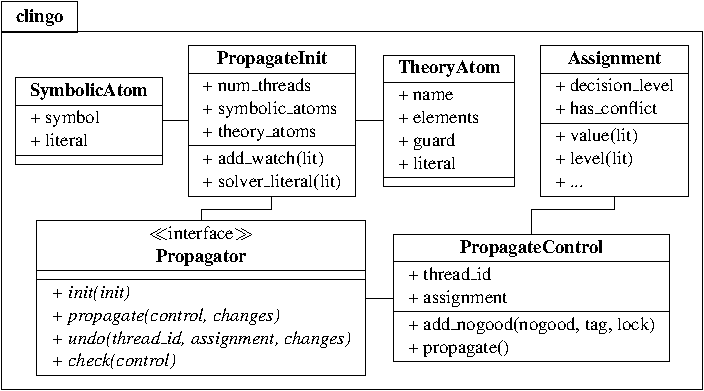
\includegraphics[width=\textwidth]{figures/python-interface}
  \caption{Class diagram of \clingo's (theory) propagator interface\label{fig:interface}}
\end{figure}
%
% To begin with,
The interface \code{Propagator} has to be implemented by each custom propagator.
After registering such a propagator with \clingo,
its functions are called during initialization and search as indicated % in the algorithm
in Figure~\ref{fig:cdcl}.
%
Function \code{Propagator.init}%
\footnote{For brevity, we below drop the qualification \code{Propagator} and use its function names unqualified.}
is called once before solving (Line~(\ref{fig:cdcl:init}) in Figure~\ref{fig:cdcl})
to allow for initializing data structures used during theory propagation.
It is invoked with a \code{PropagateInit} object providing access to symbolic (\code{SymbolicAtom}) as well as theory (\code{TheoryAtom}) atoms.
Both kinds of atoms are associated with program literals,\footnote{Program literals are also used in the \aspif\ format (see~\ref{sec:aspif}).} % ~\cite{gekakaosscwa16b}
which are in turn associated with solver literals.%
\footnote{Note that \clasp's preprocessor might associate a positive or even negative solver literal with multiple atoms.}
Program as well as solver literals are identified by non-zero integers, where positive and negative numbers represent positive or  negative literals, respectively.
In order to get notified about assignment changes, a propagator can set up watches on solver literals during initialization.

During search, function \codeClass{Propagator}{propagate} is called with a \code{PropagateControl} object
and a (non-empty) list of watched literals that got assigned in the recent round of unit propagation (Line~(\ref{fig:cdcl:propagate}) in Figure~\ref{fig:cdcl}).
The \code{PropagateControl} object can be used to inspect the current assignment, record nogoods, and trigger unit propagation.
Furthermore, to support multi-threaded solving,
its \code{thread\_id} property identifies the currently active thread,
each of which can be viewed as an independent instance of the CDCL algorithm in Figure~\ref{fig:cdcl}.%
%Hence, thread-specific state has to be associated with the \code{thread\_id}.
\footnote{%
Depending on the configuration of \clasp, threads can communicate with each other.
For example, some of the recorded nogoods can be shared.
This is transparent from the perspective of theory propagators.}
%
Function \codeClass{Propagator}{undo} is the counterpart of \codeClass{Propagator}{propagate}
and called whenever the solver retracts assignments to watched literals (Line~(\ref{fig:cdcl:undo}) in Figure~\ref{fig:cdcl}).
In addition to the list of watched literals that have been retracted (in chronological order),
it receives the identifier and the assignment of the active thread.
%
Finally, function \codeClass{Propagator}{check} is similar to \codeClass{Propagator}{propagate},
yet invoked without a list of changes.
Instead, it is (only) called on total assignments
(Line~(\ref{fig:cdcl:check}) in Figure~\ref{fig:cdcl}), independently of watches.
%
Overriding the empty default implementations of propagator methods is optional.
% Implementing the propagator methods, which default to empty implementations, is optional. % that does nothing.
For brevity, we below focus on implementations of the methods in \python,
while \lua\ or \C\ could be used as well.

For illustration,
consider Listing~\ref{prg:pigeon:propagator} giving a propagator for (half of) the pigeon-hole problem.
%
\lstinputlisting[linerange={1-10,12-39},float=t,mathescape=true,escapeinside={\#(}{\#)},basicstyle={\ttfamily\small},label={prg:pigeon:propagator},caption={Propagator for the pigeon-hole problem},language=clingo]{example/pigeon-py.lp}
%
Although this setting is constructed, it showcases central aspects
that are also relevant when implementing more complex propagators,
e.g., the \code{Pigeonator} is both stateful and can be used with multiple threads.
%
The underlying ASP encoding is given in Line~\ref{prg:pigeon:prop:rule1}:
A (choice) rule generates solution candidates by placing each of the $p$ pigeons in exactly one among $h$ holes.
While the rule commented out in Line~\ref{prg:pigeon:prop:rule2} would ensure that there is at most one pigeon per hole,
this constraint is handled by the \code{Pigeonator} class
implementing the \code{Propagator} interface (except for \code{check}) in Lines~\ref{prg:pigeon:prop:begin-init}--\ref{prg:pigeon:prop:end-undo}.
Whenever two pigeons are placed in the same hole, it adds a binary nogood forbidding the placement.
To this end,
it maintains data structures for, given a newly placed pigeon,
detecting whether there is a conflict.
%
More precisely, the propagator has two data members:
The \code{self.place} dictionary in Line~\ref{prg:pigeon:prop:member-place} maps solver literals
for \code{place}$/2$ atoms to their corresponding holes,
and the \code{self.state} list in Line~\ref{prg:pigeon:prop:member-state} stores for each solver thread its current placement of pigeons
as a mapping from holes to true solver literals for \code{place}$/2$ atoms.

Function \codeClass{Pigeonator}{init} in Lines~\ref{prg:pigeon:prop:begin-init}--\ref{prg:pigeon:prop:end-init}
sets up watches as well as the dictionaries in \code{self.place} and \code{self.state}.
%
To this end,
it traverses (symbolic) atoms over \code{place}$/2$ in Lines~\ref{prg:pigeon:prop:init:loop-atoms}--\ref{prg:pigeon:prop:init:end-loop-atoms}.
Each such atom is associated with a solver literal, % in \clasp,
obtained in Line~\ref{prg:pigeon:prop:init:map-literal}.
The mapping from the solver literal to its corresponding hole is then stored in the \code{self.place} dictionary in
Line~\ref{prg:pigeon:prop:init:map-lit-hole}.
%
In the last line of the loop, a watch is added for each solver literal at hand,
so that the solver calls \code{propagate} whenever a pigeon is placed. % in the hole as specified by the placement atom.
%
Finally, in Line~\ref{prg:pigeon:prop:init:state}, the \code{self.state} list
of placements per thread,
subject to change upon propagation and backjumping,
% Given a solving thread $i$, each state \code{self.state[$i$]} is a dictionary mapping holes to placement atoms given by their literals.
is initialized with empty dictionaries.

Function \codeClass{Pigeonator}{propagate}, given in Lines~\ref{prg:pigeon:prop:begin-prop}--\ref{prg:pigeon:prop:end-prop},
accesses \code{control.thread\_id} in Line~\ref{prg:pigeon:prop:prop:state}
to obtain the \code{holes} dictionary storing the active thread's current placement of pigeons.
% At first, in Line~\ref{prg:pigeon:prop:prop:state},
% \code{control.thread\_id} is used to obtain the dictionary storing the current thread's partial placement of pigeons.
The loop in Lines~\ref{prg:pigeon:prop:prop:begin-loop}--\ref{prg:pigeon:prop:prop:end-loop} then iterates over the list of changes,
i.e., solver literals representing newly placed pigeons.
After in Line~\ref{prg:pigeon:prop:prop:pigeon-to-hole}
determining the \code{hole} associated with a recently assigned literal,
% , the target \code{hole} associated with the current literal is obtained.
% Then,
\python's \code{setdefault} function is used to update the state:
Depending on whether \code{hole} already appears as a key in the \code{holes} dictionary,
the function either retrieves its associated literal or inserts the new literal under key \code{hole}. % into the dictionary.
While the latter case amounts to updating the placement of pigeons, the former signals a conflict,
triggered by recording a binary nogood in Line~\ref{prg:pigeon:prop:prop:add-clause}.
% In case of a conflict, the propagator adds a binary nogood in Line~\ref{prg:pigeon:prop:prop:add-clause} preventing such an invalid placement of pigeons.
Given that the solver has to resolve the conflict and backjump,
the call to \code{add\_nogood} always yields false, so that
propagation stops without processing remaining changes any further.\footnote{%
  The optional arguments \code{tag} and \code{lock} of \code{add\_nogood} can be used to control the scope and lifetime of recorded nogoods.
  Furthermore, in a propagator that does not add violated nogoods only, % but also unit-resulting nogoods
  function \code{control.propagate} can be invoked to trigger unit propagation.
  }
% Furthermore, using dictionaries \code{state[i]} and \code{place}, conflicts are detected in constant time.

Function \codeClass{Pigeonator}{undo} in Lines~\ref{prg:pigeon:prop:begin-undo}--\ref{prg:pigeon:prop:end-undo} resets a thread's placement of pigeons upon backjumping.
Similar to \codeClass{Pigeonator}{propagate}, % it is called by each solving thread.
the active thread's current placement
is obtained in Line~\ref{prg:pigeon:prop:undo:state},
and changes are traversed in Lines~\ref{prg:pigeon:prop:undo:begin-loop}--\ref{prg:pigeon:prop:undo:del}.
% The function then loops over the set of changes,
% that is, the literals corresponding to pigeons to be removed from the partial placement in Line~\ref{prg:pigeon:prop:undo:del}.
The latter correspond to retracted solver literals,
for which the condition in Line~\ref{prg:pigeon:prop:undo:test} makes sure
that exactly those stored in Line~\ref{prg:pigeon:prop:prop:setdefault} before are cleared,
thus reflecting that the \code{hole} determined in Line~\ref{prg:pigeon:prop:undo:pigeon-to-hole}
is free again.
%%
Finally,
function \code{main} in Lines~\ref{prg:pigeon:prop:begin-main}--\ref{prg:pigeon:prop:end-main} first registers the \code{Pigeonator} propagator in Line~\ref{prg:pigeon:prop:register},
and then initiates grounding and solving with \clingo.

%%% Local Variables:
%%% mode: latex
%%% TeX-master: "paper"
%%% End:


%%% Local Variables:
%%% mode: latex
%%% TeX-master: "paper"
%%% End:


\section{A case-study on ASP modulo Difference Logic}
\label{sec:case}

In this section, we develop a propagator to extend ASP with \emph{quantifier free integer difference logic} (\IDL).
The complete source code of this propagator is available in the github repository at \url{https://github.com/potassco/clingo/tree/master/examples/clingo/dl}.

In addition to the rules introduced in Section~\ref{sec:background},
we now also support rules of form
\begin{lstlisting}[mathescape,numbers=none]
  &diff{$u$-$v$} <= $d$ :- $a_{1}$,...,$a_n$,not $a_{n+1}$,...,not $a_o$
\end{lstlisting}
where $u$ and $v$ are (regular) terms,
$d$ is an integer constant,
each $a_i$ is an atom,
and $0 \leq n \leq o$.
For simplicity, we restrict the occurrence of theory atoms to rule heads.%
\footnote{More general settings are discussed in~\cite{jakaosscscwa17a} and made available at~\url{https://potassco.org/clingo}.}
%
Hence, stable models may now also include theory atoms of form `\lstinline[mathescape,literate={\[}{\{}{1}{\]}{\}}{1}]{&diff [$u$-$v$] <= $d$}'.
%
More precisely,
for a stable model $X$, let $C_X$ be the set of \emph{difference constraints} such as $u-v \leq d$ associated with theory atoms
`\lstinline[mathescape,literate={\[}{\{}{1}{\]}{\}}{1}]{&diff [$u$-$v$] <= $d$}' in $X$
and $V_X$ be the set of all (integer) variables occurring in the difference constraints in $C_X$.
%
In our case, a stable model $X$ is then \emph{\IDL-stable},
if there is a mapping from $V_X$ to the set of integers
satisfying all constraints in $C_X$.

% --------------------------------------------------------------------------------
\lstinputlisting[float=t,mathescape=true,literate={\%\%}{}{0},escapeinside={\#(}{\#)},basicstyle={\ttfamily\small},label={prg:dl:theory},caption={Theory language and main loop for difference constraints (dl.lp)},language=clingo,firstline=1]{example/dl/dl.lp}
% --------------------------------------------------------------------------------
To allow for writing difference constraints in rule heads,
we define theory~\lstinline{dl} in lines~\ref{prg:dl:theory:begin}--\ref{prg:dl:theory:end} in Listing~\ref{prg:dl:theory},
a subset of the theory~\lstinline{lc} presented in Listing~\ref{prg:lc} in Section~\ref{sec:language}.
%
The following lines~\ref{prg:dl:theory:main:begin}--\ref{prg:dl:theory:main:end} implement a customized main function.
The difference to \clingo's regular main function is that a propagator for difference constraints is registered at the beginning;
grounding and solving then follow as usual.
%
Note that the solve function in line~\ref{prg:dl:theory:solve} takes a model callback as argument.
Whenever an \IDL-stable model $X$ is found,
this callback prints the mapping satisfying the corresponding difference constraints~$C_X$.
The model $X$ (excluding theory atoms) is printed as part of \clingo's default output.
% --------------------------------------------------------------------------------
\begin{figure}[t]
\centering
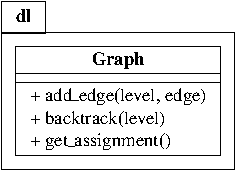
\includegraphics[]{figures/graph-interface}
\caption{Class diagram for the graph class\label{fig:class:graph}}
\end{figure}
% --------------------------------------------------------------------------------

Our exemplary propagator implements the algorithm presented in~\cite{cotmal06a}.
%
The idea is that deciding whether a set of difference constraints is satisfiable can be mapped to a graph problem.
Given a set of difference constraints, let $(V,E)$ be the weighted directed graph
where $V$ is the set of variables occurring in the constraints,
and $E$ the set of edges $(u, v, d)$ for each constraint $u-v\leq d$.
The set of difference constraints is satisfiable if the corresponding graph does not contain a negative cycle.
%
The \code{Graph} class whose interface is given in Figure~\ref{fig:class:graph} is in charge of cycle detection.
We refrain from giving the code of the \code{Graph} class and rather concentrate on describing its interface:
\begin{itemize}
\item
  Function \codeClass{Graph}{add\_edge} adds an edge of form \lstinline{(u,v,d)} to the graph. 
  If after adding the edge to the graph there is a negative cycle,
  the function returns the cycle in form of a list of edges;
  otherwise, it returns \lstinline{None}.
  Furthermore, each edge added to the graph is associated with a decision level%
  \footnote{The assignment maintains the decision level; 
    it is incremented for each decision made and decremented for each decision undone while backjumping; 
    initially, the decision level is zero.}.
  This additional information is used to backtrack to a previous state of the graph,
  whenever the solver has to backtrack to recover from a conflict.
\item
  Function \codeClass{Graph}{backtrack} takes a decision level as argument.
  It removes all edges added on that level from the graph.
  For this to work, decision levels have to be backtracked in chronological order.
  Note that the CDCL algorithm in Figure~\ref{fig:cdcl} calling our propagator also backtracks decision levels in chronological order.
\item
  As a side effect, the \code{Graph} class internally maintains an assignment of integers to nodes.
  This assignment can be turned into an assignment to the variables such that the difference constraints corresponding to the edges of the graph are satisfied.
  Function \code{get\_assignment} returns this assignment in form of a list of pairs of variables and integers.
\end{itemize}

% --------------------------------------------------------------------------------
\lstinputlisting[linerange={99-146},firstnumber=99,float=tp,mathescape=true,escapeinside={\#(}{\#)},basicstyle={\ttfamily\small},label={prg:dl:propagator},caption={Propagator for difference constraints (dl.py)},language=clingo]{example/dl/dl.py}
% --------------------------------------------------------------------------------
%
We give our exemplary propagator for difference constraints in Listing~\ref{prg:dl:propagator}.
%
It implements the \code{Propagator} interface (except for \code{check}) in Figure~\ref{fig:interface} in
lines~\ref{prg:dl:propagator:init:begin}--\ref{prg:dl:propagator:undo:end},
while featuring aspects like
incremental propagation and backtracking,
solving with multiple threads, and
multi-shot solving.
Whenever the set of edges associated with the current partial assignment of a solver induces a negative cycle
and, hence, the corresponding difference constraints are unsatisfiable,
it adds a nogood forbidding the negative cycle.
%
To this end,
it maintains data structures for, given newly added edges,
detecting whether there is a conflict.
More precisely, the propagator has three data members:
\begin{enumerate}
\item
  The \code{self.\_\_l2e} dictionary in line~\ref{prg:dl:propagator:member:l2e} maps solver literals
  for difference constraint theory atoms to their corresponding edges%
  \footnote{A solver literal might be associated with multiple edges, see Footnote~\ref{fnt:solver:literals}.},
\item
  the \code{self.\_\_e2l} dictionary in line~\ref{prg:dl:propagator:member:e2l} maps edges back to solver literals,%
  \footnote{In one solving step, the \clingo{} API guarantees that a (grounded) theory atom is associated with exactly one solver literal.
  Theory grounded in later solving steps can be associated with fresh solver literals though.}
\item
  and the \code{self.\_\_state} list in line~\ref{prg:dl:propagator:member:state} stores for each solver thread its current graph
  with the edges assigned so far.
\end{enumerate}

Function \codeClass{Propagator}{init} in lines~\ref{prg:dl:propagator:init:begin}--\ref{prg:dl:propagator:init:end}
sets up watches as well as the dictionaries in \code{self.\_\_l2e} and \code{self.\_\_e2l}.
To this end,
it traverses the theory atoms over \code{diff}$/0$ in lines~\ref{prg:dl:propagator:init:loop:begin}--\ref{prg:dl:propagator:init:loop:end}.
Note that the loop simply ignores all other theory atoms making it possible to also add propagators for other theories.
%
In lines~\ref{prg:dl:propagator:init:edge:begin}--\ref{prg:dl:propagator:init:edge:end} we extract the edge from the theory atom.%
\footnote{Here we assume that the user supplied a valid theory atom.
  A propagator for production should check validity and provide proper error messages.}
%
Each such atom is associated with a solver literal,
obtained in line~\ref{prg:dl:propagator:init:map-literal}.
The mappings between solver literals and corresponding edges are then stored in the \code{self.\_\_l2e} and \code{self.\_\_e2l} dictionaries in
lines~\ref{prg:dl:propagator:init:l2e} and~\ref{prg:dl:propagator:init:e2l}.\footnote{
  \python's \code{setdefault} function is used to update the mappings.
  Depending on whether the given \code{key} already appears in the dictionary,
  the function either retrieves the associated value or inserts and returns the second argument.}
In the last line of the loop, a watch is added for each solver literal at hand,
so that the solver calls \code{propagate} whenever the edge has to be added to the graph.

Function \codeClass{Propagator}{propagate}, given in lines~\ref{prg:dl:propagator:propagate:begin}--\ref{prg:dl:propagator:propagate:end},
accesses \code{control.thread\_id} in line~\ref{prg:dl:propagator:propagate:state}
to obtain the graph associated with the active thread.
%
The loops in lines~\ref{prg:dl:propagator:propagate:loop:begin}--\ref{prg:dl:propagator:propagate:loop:end} then iterate over the list of changes and associated edges.
In line \ref{prg:dl:propagator:propagate:add-edge} each such edge is added to the graph.
If adding the edge produced a negative cycle,
a nogood is added in line~\ref{prg:dl:propagator:propagate:add-nogood}.
Because an edge can be associated with multiple solver literals,
we use function \codeClass{Propagator}{\_\_literal}
retrieving the first solver literal associated with an edge that is true,
to construct the nogood forbidding the cycle.
%
Given that the solver has to resolve the conflict and backjump,
the call to \code{add\_nogood} always yields false,
so that propagation is stopped without processing the remaining changes any further.\footnote{%
  The optional arguments \code{tag} and \code{lock} of \code{add\_nogood} can be used to control the scope and lifetime of recorded nogoods.
  Furthermore, if a propagator adds nogoods that are not necessarily violated,
  function \code{control.propagate} can be invoked to trigger unit propagation.}

Given that each edge added to the graph in line~\ref{prg:dl:propagator:propagate:add-edge} is associated with the current decision level,
the implementation of function \codeClass{Propagator}{undo} is quite simple.
It calls function \codeClass{Graph}{backtrack} on the solver's graph to remove all edges added on the current decision level.

% --------------------------------------------------------------------------------
\begin{figure}[ht]
\centering
{\def\svgscale{.4}
%% Creator: Inkscape inkscape 0.91, www.inkscape.org
%% PDF/EPS/PS + LaTeX output extension by Johan Engelen, 2010
%% Accompanies image file 'dl.pdf' (pdf, eps, ps)
%%
%% To include the image in your LaTeX document, write
%%   \input{<filename>.pdf_tex}
%%  instead of
%%   \includegraphics{<filename>.pdf}
%% To scale the image, write
%%   \def\svgwidth{<desired width>}
%%   \input{<filename>.pdf_tex}
%%  instead of
%%   \includegraphics[width=<desired width>]{<filename>.pdf}
%%
%% Images with a different path to the parent latex file can
%% be accessed with the `import' package (which may need to be
%% installed) using
%%   \usepackage{import}
%% in the preamble, and then including the image with
%%   \import{<path to file>}{<filename>.pdf_tex}
%% Alternatively, one can specify
%%   \graphicspath{{<path to file>/}}
%% 
%% For more information, please see info/svg-inkscape on CTAN:
%%   http://tug.ctan.org/tex-archive/info/svg-inkscape
%%
\begingroup%
  \makeatletter%
  \providecommand\color[2][]{%
    \errmessage{(Inkscape) Color is used for the text in Inkscape, but the package 'color.sty' is not loaded}%
    \renewcommand\color[2][]{}%
  }%
  \providecommand\transparent[1]{%
    \errmessage{(Inkscape) Transparency is used (non-zero) for the text in Inkscape, but the package 'transparent.sty' is not loaded}%
    \renewcommand\transparent[1]{}%
  }%
  \providecommand\rotatebox[2]{#2}%
  \ifx\svgwidth\undefined%
    \setlength{\unitlength}{297.11999512bp}%
    \ifx\svgscale\undefined%
      \relax%
    \else%
      \setlength{\unitlength}{\svgscale\unitlength}%
    \fi%
  \else%
    \setlength{\unitlength}{\svgwidth}%
  \fi%
  \global\let\svgwidth\undefined%
  \global\let\svgscale\undefined%
  \makeatother%
  \begin{picture}(1,0.51534733)%
    \put(0,0){
\includegraphics[width=\unitlength,page=1]{figures/dl.pdf}}%
    \put(0.20382337,0.43268764){\color[rgb]{0,0,0}\makebox(0,0)[rb]{\smash{task}}}%
    \put(0.28459882,0.43268764){\color[rgb]{0,0,0}\makebox(0,0)[lb]{\smash{duration on machine}}}%
    \put(0.20382337,0.28459932){\color[rgb]{0,0,0}\makebox(0,0)[rb]{\smash{a}}}%
    \put(0.20382337,0.16343615){\color[rgb]{0,0,0}\makebox(0,0)[rb]{\smash{b}}}%
    \put(0.20382337,0.04227298){\color[rgb]{0,0,0}\makebox(0,0)[rb]{\smash{c}}}%
    \put(0,0){
\includegraphics[width=\unitlength,page=2]{figures/dl.pdf}}%
  \end{picture}%
\endgroup%
}
\caption{Flow shop: instance with three tasks and two machines\label{fig:fs:ins}}
\end{figure}
\begin{figure}[ht]
\centering
{\def\svgwidth{\linewidth}
%% Creator: Inkscape inkscape 0.91, www.inkscape.org
%% PDF/EPS/PS + LaTeX output extension by Johan Engelen, 2010
%% Accompanies image file 'dl-sol.pdf' (pdf, eps, ps)
%%
%% To include the image in your LaTeX document, write
%%   \input{<filename>.pdf_tex}
%%  instead of
%%   \includegraphics{<filename>.pdf}
%% To scale the image, write
%%   \def\svgwidth{<desired width>}
%%   \input{<filename>.pdf_tex}
%%  instead of
%%   \includegraphics[width=<desired width>]{<filename>.pdf}
%%
%% Images with a different path to the parent latex file can
%% be accessed with the `import' package (which may need to be
%% installed) using
%%   \usepackage{import}
%% in the preamble, and then including the image with
%%   \import{<path to file>}{<filename>.pdf_tex}
%% Alternatively, one can specify
%%   \graphicspath{{<path to file>/}}
%% 
%% For more information, please see info/svg-inkscape on CTAN:
%%   http://tug.ctan.org/tex-archive/info/svg-inkscape
%%
\begingroup%
  \makeatletter%
  \providecommand\color[2][]{%
    \errmessage{(Inkscape) Color is used for the text in Inkscape, but the package 'color.sty' is not loaded}%
    \renewcommand\color[2][]{}%
  }%
  \providecommand\transparent[1]{%
    \errmessage{(Inkscape) Transparency is used (non-zero) for the text in Inkscape, but the package 'transparent.sty' is not loaded}%
    \renewcommand\transparent[1]{}%
  }%
  \providecommand\rotatebox[2]{#2}%
  \ifx\svgwidth\undefined%
    \setlength{\unitlength}{948.00009766bp}%
    \ifx\svgscale\undefined%
      \relax%
    \else%
      \setlength{\unitlength}{\svgscale\unitlength}%
    \fi%
  \else%
    \setlength{\unitlength}{\svgwidth}%
  \fi%
  \global\let\svgwidth\undefined%
  \global\let\svgscale\undefined%
  \makeatother%
  \begin{picture}(1,0.45569621)%
    \put(0,0){
\includegraphics[width=\unitlength,page=1]{figures/dl-sol.pdf}}%
    \put(0.13924056,0.23206748){\color[rgb]{0,0,0}\makebox(0,0)[lb]{\smash{a < c < b}}}%
    \put(0,0){
\includegraphics[width=\unitlength,page=2]{figures/dl-sol.pdf}}%
    \put(0.1139241,0.18565396){\color[rgb]{0,0,0}\makebox(0,0)[rb]{\smash{1}}}%
    \put(0.1139241,0.14767931){\color[rgb]{0,0,0}\makebox(0,0)[rb]{\smash{2}}}%
    \put(0,0){
\includegraphics[width=\unitlength,page=3]{figures/dl-sol.pdf}}%
    \put(0.1139241,0.41772158){\color[rgb]{0,0,0}\makebox(0,0)[rb]{\smash{machine}}}%
    \put(0.13924056,0.36708866){\color[rgb]{0,0,0}\makebox(0,0)[lb]{\smash{a < b < c}}}%
    \put(0,0){
\includegraphics[width=\unitlength,page=4]{figures/dl-sol.pdf}}%
    \put(0.1139241,0.32067507){\color[rgb]{0,0,0}\makebox(0,0)[rb]{\smash{1}}}%
    \put(0.1139241,0.28270039){\color[rgb]{0,0,0}\makebox(0,0)[rb]{\smash{2}}}%
    \put(0,0){
\includegraphics[width=\unitlength,page=5]{figures/dl-sol.pdf}}%
    \put(0.13924056,0.41772158){\color[rgb]{0,0,0}\makebox(0,0)[lb]{\smash{solution}}}%
    \put(0,0){
\includegraphics[width=\unitlength,page=6]{figures/dl-sol.pdf}}%
    \put(0.13924056,0.0970464){\color[rgb]{0,0,0}\makebox(0,0)[lb]{\smash{b < a < c}}}%
    \put(0,0){
\includegraphics[width=\unitlength,page=7]{figures/dl-sol.pdf}}%
    \put(0.1139241,0.0506329){\color[rgb]{0,0,0}\makebox(0,0)[rb]{\smash{1}}}%
    \put(0.1139241,0.01265828){\color[rgb]{0,0,0}\makebox(0,0)[rb]{\smash{2}}}%
    \put(0.5696203,0.23206748){\color[rgb]{0,0,0}\makebox(0,0)[lb]{\smash{c < a < b}}}%
    \put(0,0){
\includegraphics[width=\unitlength,page=8]{figures/dl-sol.pdf}}%
    \put(0.5696203,0.36708846){\color[rgb]{0,0,0}\makebox(0,0)[lb]{\smash{b < c < a}}}%
    \put(0,0){
\includegraphics[width=\unitlength,page=9]{figures/dl-sol.pdf}}%
    \put(0.5696203,0.0970463){\color[rgb]{0,0,0}\makebox(0,0)[lb]{\smash{c < b < a}}}%
    \put(0,0){
\includegraphics[width=\unitlength,page=10]{figures/dl-sol.pdf}}%
    \put(0.54008433,0.36708862){\color[rgb]{0,0,0}\makebox(0,0)[rb]{\smash{18}}}%
    \put(0.54008433,0.23206754){\color[rgb]{0,0,0}\makebox(0,0)[rb]{\smash{19}}}%
    \put(0.54008433,0.09704645){\color[rgb]{0,0,0}\makebox(0,0)[rb]{\smash{16}}}%
    \put(0.98734167,0.36708862){\color[rgb]{0,0,0}\makebox(0,0)[rb]{\smash{16}}}%
    \put(0.98734167,0.23206754){\color[rgb]{0,0,0}\makebox(0,0)[rb]{\smash{20}}}%
    \put(0.98734167,0.09704645){\color[rgb]{0,0,0}\makebox(0,0)[rb]{\smash{20}}}%
  \end{picture}%
\endgroup%
}
\caption{Flow shop: solutions for all possible permutations with the total execution length in the top right corner and optimal solutions with a blue background\label{fig:fs:sol}}
\end{figure}
% --------------------------------------------------------------------------------
%
To see our propagator in action, we consider the flow shop problem,
dealing with a set of tasks $T$ that have to be consecutively executed on $m$ machines.
%
Each task has to be processed on each machine from $1$ to $m$. 
Different parts of one task are completed on each machine resulting in the completion of the task after execution on all machines is finished.
Before a task can be processed on machine $i$, it has to be finished on machine $i-1$.
The duration of different tasks on the same machine may vary.
A task can only be executed on one machine at a time and
a machine must not be occupied by more than one task at a time.
%
An (optimal) solution to the problem is a permutation of tasks so that all tasks are finished as early as possible.

Figure~\ref{fig:fs:ins} depicts a possible instance for the flow shop problem.
The three tasks \code{a}, \code{b}, and \code{c} have to be scheduled on two machines.
The colored boxes indicate how long a task has to run on a machine.
Lighter shades of the same color are for the first and darker ones for the second machine.
For example, task \code{a} needs to be processed for~$3$ time units on the first and~$4$ time units on the second machine.

% --------------------------------------------------------------------------------
\lstinputlisting[float=ht,mathescape=true,escapeinside={\#(}{\#)},basicstyle={\ttfamily\small},label={prg:fs:ins},caption={Flow shop instance (fsI.lp)},language=clingo]{example/dl/fsI.lp}
% --------------------------------------------------------------------------------
\lstinputlisting[float=ht,literate={\%\%}{}{0},linerange={1-21,23-24},mathescape=true,escapeinside={\#(}{\#)},basicstyle={\ttfamily\small},label={prg:fs:enc},caption={Encoding of flow shop using difference constraints (fsE.lp)},language=clingo]{example/dl/fsE.lp}
% --------------------------------------------------------------------------------
%
Next we encode this problem using difference constraints.
We give in Listing~\ref{prg:fs:ins} a straightforward encoding of the instance in Figure~\ref{fig:fs:ins}.
Listing~\ref{prg:fs:enc} depicts the encoding of the flow shop problem.
Following the generate, define, and test methodology of ASP,
we first generate in lines~\ref{prg:fs:perm:begin}--\ref{prg:fs:perm:end} all possible permutations of tasks,
where atoms of form \code{permutation(T,U)} encode that task~$T$ has to be executed before task~$U$.
Then, in the following lines~\ref{prg:fs:diff:begin}--\ref{prg:fs:diff:end},
we use difference constraints to calculate the duration of the generated permutation.
%
The difference constraint in line~\ref{prg:fs:permutation:seq} guarantees that the tasks are executed in the right order.
For example, $\code{(a,1)} - \code{(a,2)} \leq -d$ ensures that task~\code{a} can only be executed on machine~\code{2} if it has finished on machine~\code{1}.
Hence, variable \code{(a,2)} has to be assigned so that it is greater or equal to $\code{(a,2)}-d$ where $d$ is the duration of task \code{a} on machine \code{1}.
Similarly, $\code{(a,1)} - \code{(b,1)} \leq -d$ makes sure that task~\code{b} can only be executed on machine~\code{1} if task~\code{a} has finished on machine~\code{1}.
While the first constraint is a fact (see line~\ref{prg:fs:permutation:seq:machine}),
the latter is subject to the generated permutation of tasks (see line~\ref{prg:fs:permutation:seq:task}).
%
The difference constraint in line~\ref{prg:fs:null} ensures that all time points at which a task is started are greater than zero.
Note that this constraint is in principle redundant
but since sets of difference constraints always have infinitely many solutions
it is good practice to encode relative to a starting point.
Furthermore, note that~\code{0} is actually a variable.
In fact, the \code{Graph} class takes care of subtracting the value of variable~\code{0} from all other variables when returning an assignment
to get easier interpretable solutions.

Running encoding and instance with the \code{dl} propagator results in the following $6$ solutions
corresponding to the solutions in Figure~\ref{fig:fs:sol}.%
\footnote{Note that in each solution all tasks are executed as early as possible.
  This is no coincidence and actually guaranteed by the algorithm implemented in the \code{Graph} class.}
One for each possible permutation of tasks:
%
% --------------------------------------------------------------------------------
\lstinputlisting[numbers=none,escapechar=!,basicstyle={\ttfamily\small}]{example/dl/fsA.txt}
% --------------------------------------------------------------------------------

% --------------------------------------------------------------------------------
\lstinputlisting[float=tp,mathescape=true,literate={\%\%}{}{0},escapeinside={\#(}{\#)},basicstyle={\ttfamily\small},label={prg:dl:theory:opt},caption={Main loop for difference constraints with optimization (dlO.lp)},language=clingo,firstline=1]{example/dl/dlO.lp}
% --------------------------------------------------------------------------------
%
Finally, to find optimal solutions,
we combine the algorithms in Listing~\ref{prg:opt:main} and Listing~\ref{prg:dl:theory} to minimize the total execution time of the tasks.
The adapted algorithm is given in Listing~\ref{prg:dl:theory:opt} .
%
As with algorithm in~\ref{prg:dl:theory}, a propagator is registered before solving.
And the control flow is similar to the branch-and-bound-based optimization algorithm in Listing~\ref{prg:opt:main}
except that we now minimize the variable \code{bound};
or better the difference between variable~\code{0} and~\code{bound}
by adding the difference constraint $\code{0} - \code{bound} \leq b$ to the program in line~\ref{prg:dl:theory:opt:bound}
where $b$ is the best known execution time of the tasks as obtained from the assignment in line~\ref{prg:dl:theory:opt:get-bound} minus $1$.
To bound maximum execution time of the task,
we have to add one more line to the encoding in Listing~\ref{prg:fs:enc}:
\begin{lstlisting}[language=clingo,firstnumber=22]
  &diff { (T,M)-bound } <= -D :- duration(T,M,D).
\end{lstlisting}
This makes sure that each task ends within the given bound.
Running encoding and instance with the \code{dl} propagator results in the optimum bound~$16$ where
the obtained solution corresponds to the left of the two optimal solutions indicated by a light blue background in Figure~\ref{fig:fs:sol}:
% --------------------------------------------------------------------------------
\lstinputlisting[numbers=none,escapechar=!,basicstyle={\ttfamily\small}]{example/dl/fsO.txt}
% --------------------------------------------------------------------------------

%%% Local Variables:
%%% mode: latex
%%% TeX-master: "paper"
%%% End:


\section{Discussion}\label{sec:discussion}

Various ways of adding domain-specific information have been explored in the literature.
%
A prominent approach is to implement forms of preferential reasoning
% , like reasoning wrt inclusion-minimal models, 
by directing choices through
a given partial order on literals~\cite{cacacale96a,rogima10a,giumar12a}.
%
To some degree, this can be simulated by heuristic modifiers like
\hpre{a}{\texttt{false}}{1}
that allow for computing a (single) inclusion-minimal model.
However, as detailed in \cite{rogima10a}, enumerating all such models needs additional constraints
or downstream tester programs.
Similarly,
\cite{balduccini11b} modifies the heuristic of the ASP solver \textit{smodels} to accommodate learning from smaller instances.
See also~\cite{falepf01a,falemari07a}.
Most notably,
\cite{rintanen12a} achieves impressive results in planning by equipping a SAT solver with
planning-specific heuristics.
%
All aforementioned approaches need customized changes to solver implementations.
%
Hence, it will be interesting to investigate how these approaches can be expressed and combined in
our declarative framework.
%
Declarative approaches to incorporating control knowledge can be found in heuristic planning.
For instance, \cite{backab00a} harness temporal logic formulas, while \cite{sierra04a} also uses
dedicated predicates for controlling backtracking in a forward planner.
%
However,
care must be taken when it comes to modifying a solver's heuristics.
Although it may lead to great improvements, it may just as well lead to a degradation of search.
In fact, the restriction of choice variables may result in exponentially larger search spaces~\cite{jajuni05a}.
This issue is reflected in our choice of heuristic modifiers, 
ranging from an \texttt{init}ial bias,
over a continued yet scalable one by \texttt{factor},
to a strict preference with \texttt{level}.

To sum up,
we introduced a declarative framework for incorporating domain-specific heuristics into ASP solving.
The seamless integration into ASP's input language provides us with a general and flexible tool for
expressing domain-specific heuristics.
As such, we believe it to be the first of its kind.
Our heuristic framework offers completely new possibilities of applying, experimenting, and studying
domain-specific heuristics in a uniform setting.
Our example heuristics merely provide first indications on the prospect of our approach,
but much more systematic empirical studies are needed to exploit its full power.


%%% Local Variables: 
%%% mode: latex
%%% TeX-master: "paper"
%%% End: 

\appendix

\section{Intermediate language}
\label{sec:aspif}
\newcommand\Space{\text{\textvisiblespace}}%

To accommodate the richer input language, a more general grounder-solver interface is needed.
Although this could be left internal to \clingo~5,
it is good practice to explicate such interfaces via an intermediate language.
This also allows for using alternative downstream solvers or transformations.

Unlike the block-oriented \smodels\ format,
the \aspif\footnote{ASP Intermediate Format} format is line-based.
Notably, it abolishes the need of using symbol tables in \smodels' format\footnote{\url{http://www.tcs.hut.fi/Software/smodels}}
for passing along meta-expressions and rather allows \gringo~5 to output information as soon as it is grounded.
An \aspif\ file starts with a header, beginning with the keyword \lstinline{asp}
along with version information and optional tags:
\[\texttt{asp} \Space v_m \Space v_n \Space v_r \Space t_1 \Space \dots \Space t_k \]
where $v_m,v_n,v_r$ are non-negative integers representing the version in terms of \textit{major}, \textit{minor}, and \textit{revision} numbers,
and each $t_i$ is a tag for $k\geq 0$.
Currently, the only tag is \lstinline{incremental}, meant to set up the underlying solver for multi-shot solving.
An example header is given in line~1 of Listing~\ref{prg:ezy:a} and~\ref{aspif:diff}.
%
The rest of the file is comprised of one or more logic programs.
Each logic program is a sequence of lines of \aspif\ statements followed by a \lstinline{0}, one statement or \lstinline{0} per line, respectively.
%
Positive and negative integers are used to represent positive or  negative literals, respectively.
Hence, \lstinline{0} is not a valid literal.

Let us now briefly describe the format of \aspif\ statements and illustrate them with a
simple logic program in Listing~\ref{prg:ezy} as well as the result of grounding a subset of Listing~\ref{prg:lc}
in Listing~\ref{aspif:diff}. % below.

% ------------------------------------------------------------
\begin{figure}
\captionsetup{type=lstlisting}
%\frame%
{\begin{sublstlisting}[b]{0.4\linewidth}
\lstinputlisting[numbers=left]{code/ezy.lp}%
\caption{Logic program}
\label{prg:ezy:a}
\end{sublstlisting}}%
\hfill%\frame%
{\begin{sublstlisting}[b]{0.4\linewidth}
\lstinputlisting[numbers=right]{code/ezy.aspif}%
\caption{\aspif\ representation}
\label{prg:ezy:b}
\end{sublstlisting}}%
\caption{Representing a simple logic program in \aspif{} format}
\label{prg:ezy}
\end{figure}
% ------------------------------------------------------------
%
% --------------------------------------------------
\newcounter{DUID}%
\newcommand{\myparagraph}[1]{\par\emph{#1}}
% --------------------------------------------------
\myparagraph{Rule statements} have form
\addtocounter{DUID}{1}
\[\texttt{\theDUID} \Space H \Space B\]
in which head $H$ has form
\[h \Space m \Space a_1 \Space \dots \Space a_m\]
where
$h \in \{\texttt{0},\texttt{1}\}$ determines whether the head is a disjunction or choice,
$m \geq 0$ is the number of head elements, and
each $a_i$ is a positive literal.

Body $B$ has one of two forms:
\begin{itemize}
\item Normal bodies have form
  \[\texttt{0} \Space n \Space l_{1} \Space \dots \Space l_n\]
  where
  $n \geq 0$ is the length of the rule body, and
  each $l_i$ is a literal.
\item Weight bodies have form
  \[\texttt{1} \Space l \Space n \Space l_1 \Space w_1  \Space \dots \Space l_n \Space w_n\]
  where
  $l$ is a positive integer to denote the lower bound,
  $n \geq 0$ is the number of literals in the rule body, and
  each $l_i$ and $w_i$ are a literal and a positive integer.
\end{itemize}
All types of ASP rules are included in the above rule format.
Heads are disjunctions or choices, including the special case of singular disjunctions for representing normal rules.
As in the \smodels\ format,
aggregates are restricted to a singular body, just that in \aspif\ cardinality constraints are taken as special weight constraints.
Otherwise, a body is simply a conjunction of literals.

The three rules in Listing~\ref{prg:ezy:a} are represented by the statements in lines~2--4 of Listing~\ref{prg:ezy:b}.
For instance, the four occurrences of \lstinline{1} in line~2 capture a rule with a choice in the head, having one element, identified by \lstinline{1}.
The two remaining zeros capture a normal body with no element.
For another example,
lines~2--7 of Listing~\ref{aspif:diff} represent the four facts in lines~1 and~2 of Listing~\ref{prg:grd:diff}
along with the ones (comprising theory atoms) in line~6 of Listing~\ref{prg:grd:diff}.

\myparagraph{Minimize statements} have form
\addtocounter{DUID}{1}
\[\texttt{\theDUID} \Space p \Space n \Space l_1 \Space w_1 \Space \dots \Space l_n \Space w_n\]
where
$p$ is an integer priority,
$n \geq 0$ is the number of weighted literals,
each $l_i$ is a literal, and
each $w_i$ is an integer weight.
%
Each of the above expressions gathers weighted literals sharing the same priority $p$
from all \lstinline{#minimize} directives and weak constraints in a logic program.
As before, maximize statements are translated into minimize statements.

\myparagraph{Projection statements} result from \lstinline{#project} directives and have form
\addtocounter{DUID}{1}
\[\texttt{\theDUID} \Space n  \Space a_1 \Space \dots \Space a_n\]
where
$n \geq 0$ is the number of atoms, and
each $a_i$ is a positive literal.

\myparagraph{Output statements} result from \lstinline{#show} directives and have form
\addtocounter{DUID}{1}
\[\texttt{\theDUID} \Space m \Space s \Space n  \Space l_1 \Space \dots \Space l_n\]
where
$n \geq 0$ is the length of the condition,
each $l_i$ is a literal, and
$m\geq0$ is an integer indicating the length in bytes of string $s$
(where $s$ excludes byte `\textbackslash0' and newline).
%
The output statements in lines~5--7 of Listing~\ref{prg:ezy:b} print the symbolic representation of atom
\lstinline{a}, \lstinline{b}, or \lstinline{c}, whenever the corresponding atom is true. % , respectively.
For instance, the string `\lstinline{a}' is printed  if atom `\lstinline{1}' holds.
Unlike this,
the statements in lines~8--11 of Listing~\ref{aspif:diff} unconditionally print the symbolic representation
of the atoms stemming from the four     facts in line~1 and~2 of Listing~\ref{prg:grd:diff}.

\myparagraph{External statements} result from \lstinline{#external} directives and have form
\addtocounter{DUID}{1}
\[\texttt{\theDUID} \Space a \Space v\]
where
$a$ is a positive literal, and
$v \in \{0,1,2,3\}$ indicates free, true, false, and release.

\myparagraph{Assumption statements} have form
\addtocounter{DUID}{1}
\[\texttt{\theDUID} \Space n \Space l_1 \Space \dots \Space l_n\]
where
$n\geq 0$ is the number of literals, and
each $l_i$ is a literal.
Assumptions instruct a solver to compute      stable models such that $l_1,\dots,l_n$ hold.
They are only valid for a single solver call.

\myparagraph{Heuristic statements} result from \lstinline{#heuristic} directives and have form
\addtocounter{DUID}{1}
\[\texttt{\theDUID} \Space m \Space a \Space k \Space p  \Space n  \Space l_1 \Space \dots \Space l_n\]
where
$m\in\{0,\dots,5\}$ stands for the ($m$+1)th heuristic modifier among % in the list
\lstinline{level}, \lstinline{sign}, \lstinline{factor}, \lstinline{init}, \lstinline{true}, and \lstinline{false}, % respectively,
$a$ is a positive literal,
$k$ is % a term evaluating to 
an integer,
$p$ is a non-negative integer priority,
$n \geq 0$ is the number of literals in the condition, and
the literals $l_i$ are the condition under which the heuristic modification should be applied.

\myparagraph{Edge statements} result from \lstinline{#edge} directives and have form
\addtocounter{DUID}{1}
\[\texttt{\theDUID} \Space u \Space v \Space n  \Space l_1 \Space \dots \Space l_n\]
where
$u$ and $v$ are integers representing an edge from node $u$ to node $v$,
$n \geq 0$ is the length of the condition, and
the literals $l_i$ are the condition for the edge to be present.

Let us now turn to the theory-specific part of \aspif.
% As mentioned, the grounder ignores the theory's semantics.
Once a theory expression is grounded,
\gringo~5 % confines itself with outputting 
outputs a serial representation of its syntax tree.
To illustrate this,
we give in Listing~\ref{aspif:diff} the (sorted) result of grounding all lines of Listing~\ref{prg:lc} related to difference constraints,
viz.\ lines~2/3, 11, 15/16, and 19, as well as lines~1 and~13.

\myparagraph{Theory terms} are represented using the following statements:
\addtocounter{DUID}{1}
\begin{align}
\texttt{\theDUID} \Space \texttt{0} & \Space u \Space w \label{eq:number}\\
\texttt{\theDUID} \Space \texttt{1} & \Space u \Space n \Space s \label{eq:symbols}\\
\texttt{\theDUID} \Space \texttt{2} & \Space u \Space t \Space n \Space u_1 \Space \dots \Space u_n \label{eq:compound-term}
\end{align}
where
$n \geq 0$ is a length,
index $u$ is a non-negative integer,
integer $w$ represents a numeric term,
% ------------------------------------------------------------
\lstinputlisting[xleftmargin=0pt,label={aspif:diff},caption={\aspif\ format}]{code/d.aspif}
% ------------------------------------------------------------
%
string $s$ of length $n$ represents a symbolic term (including functions) or an operator,
integer $t$ is either \texttt{-1}, \texttt{-2}, or \texttt{-3} for tuple terms in parentheses, braces, or brackets, respectively, or an index of a symbolic term or operator, and
each $u_i$ is an integer for a theory term.
%
Statements (\ref{eq:number}), (\ref{eq:symbols}), and (\ref{eq:compound-term})
capture
numeric terms,
symbolic terms, % and function symbols, 
as well as
compound terms (tuples, sets, lists, and terms over theory operators).
% respectively.

Fifteen theory terms are given in lines~12--26 of Listing~\ref{aspif:diff}.
Each of them is identified by a unique index in the third spot of each statement.
While lines~12--20 stand for primitive entities of type (\ref{eq:number}) or (\ref{eq:symbols}),
the ones beginning with '\lstinline[mathescape=t]{9$\Space$2}' represent compound terms.
For instance, line~21 and 22 represent \lstinline{end(1)} or  \lstinline{start(1)}, respectively,
and line~23 corresponds to \lstinline{end(1)-start(1)}.

\myparagraph{Theory atoms} are represented using the following statements:
\begin{align}
\texttt{\theDUID} \Space \texttt{4} & \Space v \Space n \Space u_1 \Space \dots \Space u_n \Space m \Space l_1 \Space \dots \Space l_m \label{eq:theory-element}\\
\texttt{\theDUID} \Space \texttt{5} & \Space a \Space p \Space n \Space v_1 \Space \dots \Space v_n \label{eq:theory-atom}\\
\texttt{\theDUID} \Space \texttt{6} & \Space a \Space p \Space n \Space v_1 \Space \dots \Space v_n \Space g \Space u_1 \label{eq:theory-atom-bounded}
\end{align}
where
$n \geq 0$ and $m \geq 0$ are lengths,
index $v$ is a non-negative integer,
$a$ is a positive literal or \texttt{0} for directives,
each $u_i$ is an integer for a theory term,
each $l_i$ is an integer for a literal,
integer~$p$ refers to a symbolic term,
each $v_i$ is an integer for a theory atom element, and
integer~$g$ refers to a theory operator.
%
Statement (\ref{eq:theory-element}) captures elements of theory atoms and directives, and
statements (\ref{eq:theory-atom}) and (\ref{eq:theory-atom-bounded}) refer to the latter.
% capture theory atoms and directives.

For instance,
line~27 captures the (single) theory element  in `\lstinline+{ end(1)-start(1) }+',
and
line~29 represents the theory atom `\lstinline[morekeywords={&diff},alsoletter={\&}]+&diff { end(1)-start(1) } <= 200+'.

\myparagraph{Comments} have form
\addtocounter{DUID}{1}
\[\texttt{\theDUID} \Space s\]
where $s$ is a string not containing a newline.

The \aspif\ format constitutes the default output of \gringo~5.
With \clasp~3.2,
ground logic programs can be read in both \smodels\ and \aspif\ format.
%%% Local Variables:
%%% mode: latex
%%% TeX-master: "paper"
%%% End:


\bibliographystyle{plain}
% \bibliography{lit,akku,procs}
\begin{thebibliography}{10}

% \bibitem{Acuna2009}
% V.~Acu{\~{n}}a, F.~Chierichetti, V.~Lacroix, A.~Marchetti-Spaccamela, M.~Sagot, L.~Stougie.
% \newblock {Modes and cuts in metabolic networks: Complexity and algorithms}.
% \newblock {\em Biosystems}, 95(1):51--60, 2009.

\bibitem{anbole13a}
C.~Ans{\'o}tegui, M.~Bonet, J.~Levy.
\newblock {SAT}-based {MaxSAT} algorithms.
\newblock {\em Artificial Intelligence}, 196:77--105, 2013.

\bibitem{baral02a}
C.~Baral.
\newblock {\em Knowledge Representation, Reasoning and Declarative Problem Solving}.
\newblock Cambridge, 2003.

\bibitem{Becker2007}
S.~Becker, A.~Feist, M.~Mo, G.~Hannum, B.~Palsson, M.~Herrgard.
\newblock {Quantitative Prediction of Cellular Metabolism with Constraint-based Models: The COBRA Toolbox}.
\newblock {\em Nature Protocols}, 2(3):727--738, 2007.

\bibitem{coevgeprscsith13a}
G.~Collet, D.~Eveillard, M.~Gebser, S.~Prigent, T.~Schaub, A.~Siegel, S.~Thiele.
\newblock Extending the metabolic network of {E}ctocarpus siliculosus using answer set programming.
\newblock 
% In P.~Cabalar and T.~Son, editors, {\em Proceedings of the Twelfth International Conference on Logic Programming and Nonmonotonic Reasoning (LPNMR'13)}, volume 8148 of {\em Lecture Notes in Artificial Intelligence}, 
{\em Proceedings LPNMR},
245--256. Springer, 2013.

\bibitem{dantzig63a}
G.~Dantzig.
\newblock {\em Linear Programming and Extensions}.
\newblock Princeton, 1963.

% \bibitem{ebhahe04a}
% O.~Ebenhöh, T.~Handorf, R.~Heinrich.
% \newblock Structural analysis of expanding metabolic networks.
% \newblock {\em Genome Informatics}, 15(1):35--45, 2004.

\bibitem{Ebrahim2013}
A.~Ebrahim, J.~Lerman, B.~Palsson, D.~Hyduke.
\newblock {COBRApy: COnstraints-Based Reconstruction and Analysis for Python.}
\newblock {\em BMC Systems Biology}, 7:74, aug 2013.

\bibitem{gekakaosscwa16a}
M.~Gebser, R.~Kaminski, B.~Kaufmann, M.~Ostrowski, T.~Schaub, P.~Wanko.
\newblock Theory solving made easy with clingo~5.
\newblock 
% In M.~Carro and A.~King, editors, {\em Technical Communications of the Thirty-second International Conference on Logic Programming (ICLP'16)}, volume~52, 
{\em Technical Comm.\ ICLP},
2:1--2:15. 
% Open Access Series in Informatics
OASIcs, 2016.

\bibitem{gekakarosc15a}
M.~Gebser, R.~Kaminski, B.~Kaufmann, J.~Romero, T.~Schaub.
\newblock Progress in clasp series 3.
\newblock 
% In F.~Calimeri, G.~Ianni, and M.~Truszczy{\'n}ski, editors, {\em Proceedings of the Thirteenth International Conference on Logic Programming and Nonmonotonic Reasoning (LPNMR'15)}, volume 9345 of {\em Lecture Notes in Artificial Intelligence}, 
{\em Proceedings LPNMR},
368--383. Springer, 2015.

\bibitem{gellif91a}
M.~Gelfond, V.~Lifschitz.
\newblock Classical negation in logic programs and disjunctive databases.
\newblock {\em New Generation Computing}, 9:365--385, 1991.

\bibitem{haebhe05a}
T.~Handorf, O.~Ebenhöh, R.~Heinrich.
\newblock Expanding metabolic networks: Scopes of compounds, robustness, and evolution.
\newblock {\em J.\ of Molec.\ Evolution}, 61(4):498--512, 2005.

\bibitem{laten2014a}
M.~Latendresse.
\newblock Efficiently gap-filling reaction networks.
\newblock {\em BMC bioinformatics}, 15(1):225, 2014.

\bibitem{marzom16a}
C.~Maranas, A.~Zomorrodi.
\newblock {\em Optimiz.\ methods in metabolic networks}.
\newblock Wiley, 2016.

\bibitem{Orth2010}
J.~Orth, B.~Palsson.
\newblock {Systematizing the generation of missing metabolic knowledge.}
\newblock {\em Biotechnology and bioengineering}, 107(3):403--12, oct 2010.

% \bibitem{orthpa10a}
% J.~Orth, I.~Thiele, B.~Palsson.
% \newblock What is flux balance analysis?
% \newblock {\em Nature biotechnology}, 28(3):245--248, 2010.

\bibitem{ostsch12a}
M.~Ostrowski, T.~Schaub.
\newblock {ASP} modulo {CSP}: The clingcon system.
\newblock {\em Theory and Practice of Logic Programming}, 12(4-5):485--503, 2012.

% \bibitem{potassco}
% Potassco website.
% \newblock http://potassco.org.

\bibitem{prcodideetdaevthcabosito14a}
S.~Prigent, G.~Collet, S.~Dittami, L.~Delage, F.~{Ethis de Corny}, O.~Dameron, D.~Eveillard, S.~Thiele, J.~Cambefort, C.~Boyen, A.~Siegel, T.~Tonon.
\newblock The genome-scale metabolic network of ectocarpus siliculosus (ectogem): a resource to study brown algal physiology and beyond.
\newblock {\em The Plant Journal}, 80(2):367–381, 2014.

\bibitem{Prigent2017}
S.~Prigent, C~.Frioux, S.~Dittami, S.~Thiele, A.~Larhlimi, G.~Collet, F.~Gutknecht, J.~Got, D.~Eveillard, J.~Bourdon, F.~Plewniak, T.~Tonon, A.~Siegel.
\newblock {Meneco, a Topology-Based Gap-Filling Tool Applicable to Degraded Genome-Wide Metabolic Networks}.
\newblock {\em PLOS Computational Biology}, 13(1):e1005276, jan 2017.

\bibitem{Reed2003}
J.~Reed, T.~Vo, C.~Schilling, B.~Palsson.
\newblock {An expanded genome-scale model of Escherichia coli K-12 (iJR904 GSM/GPR).}
\newblock {\em Genome Biology}, 4(9):R54, 2003.

\bibitem{SatishKumar2007}
V.~{Satish Kumar}, M.~Dasika, C.~Maranas.
\newblock {Optimization based automated curation of metabolic reconstructions}.
\newblock {\em BMC Bioinformatics}, 8(1):212, 2007.

\bibitem{schthi09a}
T.~Schaub, S.~Thiele.
\newblock Metabolic network expansion with {ASP}.
\newblock
% In P.~Hill and D.~Warren, editors, {\em Proceedings of the Twenty-fifth International Conference on Logic Programming (ICLP'09)}, volume 5649 of {\em Lecture Notes in Computer Science}, 
{\em Proceedings ICLP},
312--326. Springer, 2009.

\bibitem{siniso02a}
P.~Simons, I.~Niemelä, T.~Soininen.
\newblock Extending and implementing the stable model semantics.
\newblock {\em Artificial Intelligence}, 138(1-2):181--234, 2002.

\bibitem{Thiele2014}
I.~Thiele, N.~Vlassis, R.~Fleming.
\newblock {fastGapFill: efficient gap filling in metabolic networks.}
\newblock {\em Bioinformatics}, 30(17):2529--2531, sep 2014.

\bibitem{Vitkin2012}
E.~Vitkin, T.~Shlomi.
\newblock {MIRAGE: a functional genomics-based approach for metabolic network model reconstruction and its application to cyanobacteria networks.}
\newblock {\em Genome Biology}, 13(11):R111, 2012.

\end{thebibliography}

%%% Local Variables:
%%% mode: latex
%%% TeX-master: "paper"
%%% End:

\end{document}

%%% Local Variables:
%%% mode: latex
%%% TeX-master: t
%%% End:

